\providecommand{\toplevelprefix}{../..}  %
\documentclass[../../book-main_es.tex]{subfiles}

\begin{document}

\chapter{Representaciones consistentes y autoconsistentes}
\label{ch:consistent-representations}

\begin{quote}
    \hfill  ``{\em Hacer todo lo más simple posible,
    pero no más simple}.''

    $~$\hfill -- Albert Einstein
\end{quote}

\vspace{5mm}

En los capítulos anteriores, hemos argumentado que el objetivo fundamental del aprendizaje es
\textit{identificar} una distribución de datos con un soporte de baja dimensión y
\textit{transformarla} en una representación compacta y estructurada. Esto implica
dos problemas relacionados:
\begin{enumerate}
    \item \textbf{Aprendizaje de distribuciones:} ¿Cómo podemos determinar la
        distribución
        de los datos $\vX$ para permitir un muestreo o una generación generalizables?
    \item \textbf{Aprendizaje de representaciones:} ¿Cómo mapeamos los datos $\vX$ a
        una representación compacta y estructurada $\vZ$, de tal manera que la
        representación
        sea suficiente para reconstruir $\vX$?
\end{enumerate}
En los \Cref{ch:denoising,ch:lossy-compression}, hemos desarrollado una solución computacional completa
para
el problema del aprendizaje de distribuciones en el contexto de distribuciones de datos generales, basada en el
proceso de eliminación de ruido por difusión. %
%It uses data samples $\vx$ to learn the score
%function $\nabla \log p_t(\vx_t)$ of the noisy data distribution.
%Also in \Cref{ch:denoising},
En el \Cref{ch:lossy-compression}, hemos definido una
función objetivo basada en la compresión,
la ganancia de información, cuya maximización conduce a representaciones compactas y
estructuradas.
Y en el \Cref{ch:deep-networks}, hemos visto que las capas de las arquitecturas populares de redes profundas
pueden interpretarse como pasos de optimización incrementales
hacia la maximización de la ganancia de información. Esto nos permite presentar
una solución con fundamentos matemáticos al problema del aprendizaje de representaciones.

%Let us then preview the representation learning methodology we will
% introduce in
%the chapter.
%As we have mentioned, a fundamental approach to learning a good representation
%of a high-dimensional distribution with intrinsic low-dimensional structures
%is through {\em compression}. To make the
%goal of compression measurable and computable, it can be done
%explicitly by learning a coding scheme that minimizes the coding
% rate (entropy) or maximizes the information gain (coding rate
%reduction). In this context, the fundamental role of a deep neural
%network is to realize a certain iterative optimization algorithm that
%incrementally optimizes the learned representations in terms of those measures:
%\begin{equation}
%  f\colon \X
%  \xrightarrow{\hspace{1mm} f^0 \hspace{1mm}} \Z^0 \rightarrow \cdots
%  \rightarrow \Z^\ell \xrightarrow{\hspace{1mm} f^\ell \hspace{1mm}}
%  \Z^{\ell+1} \rightarrow  \cdots \to \Z^L = \Z.
%\end{equation}
%In the preceding chapter, we have shown that main architectural
%characteristics of almost all popular deep networks (ResNet, CNN, and
%Transformer) can be derived and interpreted from this perspective.

Sin embargo, cuando intentamos alcanzar un objetivo determinado mediante
la optimización, no hay garantía de que la solución $\Z$ encontrada
al final mediante la optimización voraz sea la solución correcta. De hecho, incluso si
el proceso de optimización logra encontrar la solución óptima global
$\Z^*$, no hay garantía de que dicha solución corresponda
a una representación completa de la distribución de los datos.\footnote{Esto
    podría deberse a muchas razones: por ejemplo, es posible que los datos disponibles para
    aprender la distribución no sean suficientes, o que la formulación
    del programa de optimización no tenga en cuenta algunas restricciones
o condiciones adicionales.} Por lo tanto, una pregunta que queda pendiente es:
¿cómo podemos asegurarnos de que la representación aprendida de la distribución de los datos sea
correcta o lo suficientemente buena?

Por supuesto, la única forma de verificar esto es comprobar si existe
una función de decodificación, digamos $g$, capaz de decodificar la representación aprendida
para reproducir los datos originales (su distribución) con suficiente precisión:
\begin{equation}
    \X
    \xrightarrow{\hspace{1mm} \mathcal{E} = f \hspace{1mm}} \Z
    \xrightarrow{\hspace{1mm} \mathcal{D} = g \hspace{1mm}} \hat{\X}
\end{equation}
en términos de alguna medida de similitud:
\begin{equation}
    d(\X, \hat \X).
\end{equation}
Esto nos lleva al concepto de {\em representación consistente}. Como
ya hemos mencionado brevemente en el
\Cref{ch:intro} (véase la \Cref{fig:autoencoder}), la {\em autocodificación},
que integra los
procesos de codificación y decodificación, constituye un marco natural para el aprendizaje
de dicha representación. Hemos estudiado algunos casos especiales importantes
en el \Cref{ch:classic-models} donde los soportes de la distribución son
lineales por tramos. En
este capítulo, en la \Cref{sec:consistent-representation}, estudiaremos cómo
extender el autocodificador a clases más generales de distribuciones cuyos
soportes son no lineales, tal como se ilustra en la figura
\ref{fig:manifold-autoencoding}, al tiempo que se garantiza la consistencia
entre $\X$ y $\hat \X$.
\begin{figure}
    \centering
    
\includegraphics[width=0.8\linewidth]{chapters/chapter6/figs/manifolds-autoencoding.png}
    \caption{Aprender una buena representación de autocodificación para una distribución general
        cuyos soportes se encuentran en una mezcla de subvariedades de baja dimensión.
        Obsérvese que, además de aprender una buena
        representación mediante una aplicación $f(\x, \theta)$ en un enfoque de extremo a extremo
        tal como lo hicimos en \Cref{ch:deep-networks}, queremos asegurarnos
        de que la representación así aprendida pueda ser decodificada, mediante una
        mapeo «inverso» $g(\z, \eta)$, para volver a aproximar la
    distribución de datos original.}
    \label{fig:manifold-autoencoding}
\end{figure}

Teniendo en cuenta este formalismo clásico de autocodificación, surge una pregunta lógica:
\textit{¿Dónde termina el aprendizaje de distribuciones y dónde comienza el aprendizaje de representaciones?}
%The advantages of having a structured representation are clear---it reveals
%intrinsic low-dimensional structures of the data distribution and facilitates
%subsequent tasks such as classification and generation---and if we
% can perfectly
%reconstruct the data $\vX$ from the representation $\vZ$, as representation
%learning entails, then we have technically
%solved distribution learning.
%In fact, many of the classical representation
%learning approaches that we will mention in this chapter were originally
%developed as approaches for generation.
Como veremos, la respuesta %
%as to why distribution learning and representation learning should be
%conceived as separate problems
Como veremos, la respuesta se reduce a la \textit{eficiencia}. Por lo general, resulta mucho más
eficaz, tal y como demuestra la práctica moderna, aprender una representación compacta
de la distribución de datos a modo de «preparación» de la distribución,
y solo entonces llevar a cabo el aprendizaje de la distribución sobre la representación así obtenida.
Esta es la metodología predominante en los problemas prácticos.
Demostraremos los vínculos entre los fundamentos que hemos desarrollado en
\Cref{ch:lossy-compression,ch:deep-networks}
y los últimos avances en \Cref{sec:RAE},
% \Cref{sec:SimDINO}, where we describe ``open-loop'' representation learning
% in SimDINO, and in \Cref{sec:RAE-implement},
donde el marco del «autocodificador de representaciones» muestra cómo las representaciones aprendidas en bucle abierto
(que analizamos en \Cref{sec:SimDINO} y que
revisaremos)
%learned from DINO/SimDINO 
pueden combinarse con un decodificador simple y un proceso de difusión en el espacio $\vZ$ para
permitir el aprendizaje y el muestreo de representaciones de manera eficiente y simultánea.

Más fundamentalmente, en muchos escenarios de aprendizaje prácticos y naturales,
puede resultar difícil o incluso imposible comparar las distribuciones de
los datos $\X$ y $\hat \X$. La única opción que nos queda es
comparar la característica aprendida $\Z$ con su imagen $\hat \Z$ bajo el
codificador $f$:
\begin{equation}
    \X
    \xrightarrow{\hspace{1mm} \mathcal{E} = f \hspace{1mm}} \Z
    \xrightarrow{\hspace{1mm} \mathcal{D} = g \hspace{1mm}} \hat{\X}
    \xrightarrow{\hspace{1mm} \mathcal{E} = f \hspace{1mm}} \hat \Z
\end{equation}

Esto nos lleva al concepto de una {\em representación autoconsistente}.
En \Cref{sec:self-consistency}, estudiaremos cuándo y cómo podemos
aprender una representación consistente imponiendo la autoconsistencia
entre $\Z$ y $\hat \Z$ únicamente a través de un marco de transcripción de bucle cerrado.

Además, en muchos escenarios de aprendizaje prácticos y naturales,
normalmente no disponemos de suficientes muestras de la distribución de los datos
disponibles todas a la vez. Por ejemplo, los animales y los seres humanos desarrollan su
memoria visual mediante la incorporación continua de pequeñas dosis de observaciones
a lo largo de sus vidas. En \Cref{sec:continuous}, estudiaremos cómo
ampliar el marco de transcripción de bucle cerrado para aprender una
representación autoconsistente en un entorno de {\em aprendizaje continuo}.

Por supuesto, una de las razones fundamentales por las que queremos identificar las
estructuras de baja dimensión en una distribución de datos y encontrar una buena
representación es facilitar el uso de los datos para diversas tareas
de inteligencia, como la clasificación, la completación y la predicción.
Por lo tanto, la representación conjunta resultante $(\x, \z)$ debe
estructurarse de la manera más adecuada para estas tareas. En el
siguiente capítulo, veremos
cómo se puede estructurar la representación aprendida para facilitar
las tareas de finalización o generación condicionadas.

\section{El aprendizaje de representaciones
consistentes}\label{sec:consistent-representation}

A continuación ofrecemos una definición formal de las representaciones consistentes, que
están estrechamente relacionadas con el concepto de autocodificación. %
\begin{definition}[Representaciones consistentes]\label{def:bidirectional_rep}
    Dados los datos \(\vX\), una \textit{representación consistente} es un par
    de funciones \((f \colon \cX \to \cZ, g \colon \cZ \to \cX)\), tal
    que las \textit{características} \(\vZ = f(\vX)\) son compactas y
    estructuradas, y la \textit{autocodificación}
    \begin{equation}
        \hat{\vX} \doteq g(\vZ) = g(f(\vX))
    \end{equation}
    es \textit{cercano} a \(\vX\) según una de las
    dos medidas siguientes:
    \begin{enumerate}
        \item Decimos que es consistente \textit{por muestra} si \(\vX
            \approx \hat{\vX}\) en una determinada norma con alta probabilidad.
        \item Decimos que la representación es \textit{distribucionalmente
            consistente} si \(\Law(\vX) \approx \Law(\hat{\vX})\).
    \end{enumerate}
\end{definition}

Los lectores más perspicaces habrán notado que, si no imponemos ciertos
requisitos a la representación $\Z$ que buscamos, el problema anterior tiene
una solución trivial: ¡basta con elegir las funciones $f$ y $g$
para que sean la aplicación identidad! Por lo tanto, el verdadero propósito de buscar una
autocodificación es garantizar que el $\Z$ así obtenido sea a la vez más
compacto y más estructurado que $\X$.
%First, for compactness, $\Z$
%should better reveal the intrinsic low-dimensionality of $\X$.
Como hemos visto en el \Cref{ch:deep-networks},
basta con diseñar la representación de manera que se maximice la reducción de la tasa
\begin{equation}
    \Delta R_{\epsilon}(\Z).
\end{equation}%
%Second, the main purpose of
%learning a good representation of the data distribution is to
%facilitate tasks that exploit the low-dimensionality of its
%distribution. Hence, the distribution of $\Z$ should be better
%structured. For example, the distribution of $\Z$ is piecewise linear
%or Gaussian, and its components are largely incoherent or
% independent. These independent components can represent different clusters or
%classes and can also easily be used as conditions for decoding the
%corresponding data $\x$.
Según la definición de representación consistente, se requiere que
la representación $\Z$ sea suficiente para reconstruir la distribución de datos original
$\X$ con cierto grado de precisión. Para la consistencia por muestra,
una opción habitual es minimizar el error de reconstrucción esperado:
\begin{equation}
    d(\X, \hat \X) = \mathbb{E}[\|\X - \hat\X\|_2^2].
\end{equation}
Para garantizar la coherencia distribucional, una opción habitual consiste en minimizar una
determinada distancia distributiva, como la divergencia KL
\footnote{Cabe señalar que, en el caso de distribuciones sin
    soporte común---algo habitual en las distribuciones degeneradas---la divergencia KL
    puede incluso no estar bien definida. De hecho, gran parte de la literatura sobre
    aprendizaje de distribuciones intenta abordar esta dificultad técnica
    sustituyéndola o aproximándola con algo bien definido y
que se pueda calcular de manera eficiente.}:
\begin{equation}
    d(\X, \hat \X) = \mathcal{D}_{KL}(\X\|\hat\X).
\end{equation}

Por lo tanto, dejando de lado los aspectos computacionales, cuando 
buscamos una buena autocodificación para una distribución de datos
$\X$, conceptualmente intentamos encontrar un codificador $f$ y
un decodificador $g$ tales que
\begin{equation}
    \min_{f, g} [- \Delta R_{\epsilon}(\Z) + d(\X, \hat \X)].
    \label{eqn:autoencode-objective-ch5}
\end{equation}
Obsérvese que el error de cuantificación $\epsilon$ actúa como parámetro de compensación
en esta relajación lagrangiana.

En el resto de esta sección, estudiaremos cómo resolver este tipo de
problemas de autocodificación bajo diferentes condiciones, desde casos simples e
ideales hasta condiciones cada vez más complejas y realistas.
Concluiremos con una instanciación eficiente de
\eqref{eqn:autoencode-objective-ch5} (en la \Cref{sec:RAE}) que
garantiza que el espacio de representación $\vZ$ sea compacto y estructurado, al tiempo que
permite una reconstrucción precisa y un muestreo eficiente.

\subsection{Autocodificación lineal mediante PCA}% or Online PCA}

Según \cite{Baldi2011}, el término «autocodificador» fue
introducido por primera vez por Hinton y Rumelhart \cite{Rumelhart1986} con el fin de que se pudiera
aprender una representación profunda mediante retropropagación (BP) de
manera autosupervisada; la reconstrucción de los datos originales constituye la
tarea de autosupervisión. Sin embargo, el concepto mismo de buscar una
representación compacta y coherente tiene sus raíces en muchos estudios clásicos.
Como ya hemos visto en el \Cref{ch:classic-models}, el PCA clásico,
el ICA y el aprendizaje de diccionarios dispersos comparten un objetivo similar.
La única diferencia es que, cuando la distribución de los datos subyacentes es
simple (lineal e independiente), las correspondencias de codificación o 
decodificación resultan fáciles de representar y aprender: no es necesario 
que sean profundas y, a menudo, pueden calcularse en forma cerrada o
mediante un algoritmo explícito.
Resulta instructivo observar cómo se aplica el concepto de consistencia que hemos
definido en el caso sencillo del PCA:
aquí, las correspondencias de codificación y decodificación consistentes vienen dadas por una transformación lineal
de una sola capa:
\begin{equation}
    \X \xrightarrow{\hspace{2mm} \mathcal{E} = \vU^\top \hspace{2mm}}
    \Z \xrightarrow{\hspace{2mm} \mathcal{D} = \vU \hspace{2mm}}   \hat{\X},
    \label{eqn:autoencoding-PCA-2}
\end{equation}
donde $\vU \in \mathbb{R}^{D\times d}$, normalmente con $d\ll D$. Por lo tanto,
$\vU^\top $ representa una proyección desde un espacio de mayor dimensión
$\mathbb{R}^{D}$  a uno de menor dimensión $\mathbb{R}^{d}$, tal como se ilustra en
la \Cref{fig:AE}.
\begin{figure}
    \centering
    
\includegraphics[width=0.5\linewidth]{\toplevelprefix/chapters/chapter6/figs/autoencoder.png}
    \caption{Ilustración de un autocodificador típico, como el PCA, que busca
    una representación de baja dimensión $\z$ para datos de alta dimensión $\vx$.}
    \label{fig:AE}
\end{figure}

Como vimos en \Cref{ch:classic-models}, cuando la distribución de $\vx$ se
apoya efectivamente en un subespacio de baja dimensión $\vU_o$, la compacidad de
la representación
$\vz$ generada por $\mathcal{E}$ es una consecuencia directa de estimar
correctamente (y garantizar) la dimensión de este subespacio.
Recordemos que el descenso por gradiente sobre el criterio de reconstrucción produce exactamente
estas correspondencias consistentes por muestra: de hecho, la solución óptima
al problema
\begin{equation}\label{eq:pca-reconstruction-ch5}
    \min_{\vU^\top \vU = \vI}\, \bE_{\vx}\left[\norm*{\vx
    - \vU\vU^\top \vx}_2^2\right]
\end{equation}
coincide exactamente con $\vU_o$ cuando la dimensión de la representación es
suficientemente grande. En este caso, obtenemos consistencia por muestra
de manera automática, ya que esto garantiza que $\vU_o\vU_o^\top \vx = \vx$.
Nótese que, en el caso del PCA, el término de reducción de la tasa en
\eqref{eqn:autoencode-objective-ch5} queda sin efecto, ya que la regularización
sobre la representación $\Z$ buscada es explícita: abarca todo el
subespacio de menor dimensión\footnote{En este caso, se puede considerar que $\Delta R = 0$}.

\subsection{PCA no lineal y 
autocodificación}\label{sub:nonlinear-pca}\label{sec:NLPCA}
Por supuesto, es de esperar que las cosas ya no sean tan sencillas
cuando nos enfrentemos a distribuciones más complejas cuyas estructuras subyacentes
de baja dimensión sean no lineales.

\paragraph{Datos en una subvariedad no lineal.} Por lo tanto, para ir más allá de la
estructura lineal que aborda el PCA, podemos suponer que la distribución de los datos
se encuentra en una subvariedad (suave) $\mathcal{M}$. La
dimensión intrínseca de la subvariedad, digamos $d$, suele ser mucho
menor que la
dimensión del espacio circundante $\mathbb{R}^D$. Desde esta perspectiva geométrica,
normalmente queremos encontrar una aplicación no lineal $f$ tal que
la variedad resultante
$f(\mathcal{M})$ sea aplanada, como se ilustra en el ejemplo mostrado en
\Cref{fig:idealized_interpolation}. El espacio de características $\vz$ resultante
suele ser
más compacto (de menor dimensión) que el espacio $\vx$ y la
variedad es plana.
Desde la perspectiva estadística, que es complementaria a la perspectiva geométrica
pero distinta de ella en general, tal vez también queramos asegurarnos de que la distribución de los datos
en $\mathcal{M}$ se corresponda con una distribución suficientemente regular
en el espacio $\vz$, como por ejemplo una distribución gaussiana o uniforme (con
un soporte de muy baja dimensión).
%These two properties ensure that sampling and interpolation in the
% $\vz$-space are as easy as possible, and they are mathematical
% formalizations of the desirable
%notions of compact and structured features in the low-dimensional manifold
%model for the data distribution.
En general, el problema de aprender un mapeo de autocodificación de este tipo para esta clase
de distribuciones de datos se conoce como {\em análisis de componentes principales no lineal}
(NLPCA).

\begin{figure}
    \centering
    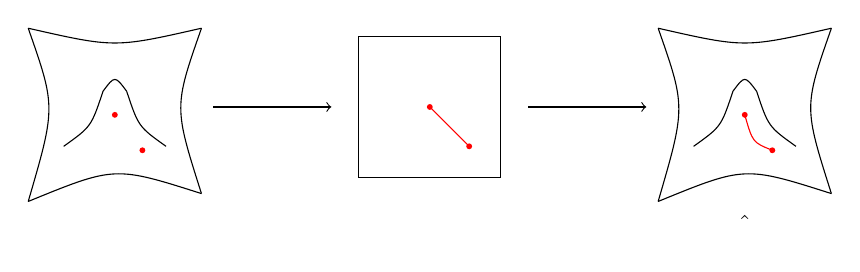
\begin{tikzpicture}
        \draw (-0.1, -0.2) .. controls (1, 0.25) .. (2.1, -0.1);
        \draw (2.1, -0.1) .. controls (1.75, 1) .. (2.1, 2);
        \draw (2.1, 2) .. controls (1, 1.75) .. (-0.1, 2);
        \draw (-0.1, 2) .. controls (0.25, 1) .. (-0.1, -0.2);

        \draw (0.35, 0.5) .. controls (0.7, 0.75) .. (0.85, 1.2);
        \draw (0.85, 1.2) .. controls (1.0, 1.4) .. (1.15, 1.2);
        \draw (1.15, 1.2) .. controls (1.3, 0.75) .. (1.65, 0.5);

        \node[fill, red, circle, inner sep=0.75pt] at (1, 0.9) {};
        \node[fill, red, circle, inner sep=0.75pt] at (1.35, 0.45) {};

        \node at (1, -0.5) {\(\x\)};

        \draw[->] (2.25, 1) -- (3.75, 1);
        \node at (3, 1.25) {\(\fl\)};

        \draw (4.1, 0.1) -- (5.9, 0.1);
        \draw (5.9, 0.1) -- (5.9, 1.9);
        \draw (5.9, 1.9) -- (4.1, 1.9);
        \draw (4.1, 1.9) -- (4.1, 0.1);

        \node[fill, red, circle, inner sep=0.75pt] at (5, 1) {};
        \node[fill, red, circle, inner sep=0.75pt] at (5.5, 0.5) {};

        \draw[red] (5, 1) -- (5.5, 0.5);

        \node at (5, -0.5) {\(\z\)};

        \draw[->] (6.25, 1) -- (7.75, 1);
        \node at (7, 1.25) {\(\re\)};

        \draw (7.9, -0.2) .. controls (9, 0.25) .. (10.1, -0.1);
        \draw (10.1, -0.1) .. controls (9.75, 1) .. (10.1, 2);
        \draw (10.1, 2) .. controls (9, 1.75) .. (7.9, 2);
        \draw (7.9, 2) .. controls (8.25, 1) .. (7.9, -0.2);

        \draw (8.35, 0.5) .. controls (8.7, 0.75) .. (8.85, 1.2);
        \draw (8.85, 1.2) .. controls (9.0, 1.4) .. (9.15, 1.2);
        \draw (9.15, 1.2) .. controls (9.3, 0.75) .. (9.65, 0.5);

        \node[fill, red, circle, inner sep=0.75pt] at (9, 0.9) {};
        \node[fill, red, circle, inner sep=0.75pt] at (9.35, 0.45) {};

        \draw[red] (9, 0.9) .. controls (9.1, 0.55) .. (9.35, 0.45);

        \node at (9, -0.5) {\(\hat{\x}\)};
    \end{tikzpicture}
    \caption{Representación de la interpolación mediante aplanamiento de variedad
        en una variedad en \(\R^{3}\) de dimensión \(d = 2\). Para interpolar
        dos puntos en la variedad de datos, se mapean estos a través de la aplicación de aplanamiento
        \(\fl\) al espacio aplanado, se toman sus interpolantes convexas
        y luego se mapean estos de vuelta a la variedad de datos a través de la
    aplicación de reconstrucción \(\re\).}
    \label{fig:idealized_interpolation}
\end{figure}

\paragraph{Un intento clásico mediante una red de dos capas.} Como hemos
visto anteriormente, en el caso del PCA, basta con una red neuronal lineal
de una sola capa. Sin embargo, esto ya no es así en el caso del NLPCA. En 1991, Kramer
\cite{Kramer1991NonlinearPC}  propuso resolver el NLPCA utilizando una red neuronal de dos capas
para representar la función de codificación $f$ (o su inversa $g$) basándose
en la propiedad de representación universal de las redes de dos capas con activación sigmoide:
\begin{equation}
    \z = \vW_2 \sigma(\vW_1\x +\vb),
\end{equation}
donde $\sigma(\spcdot)$ es la función sigmoide:
\begin{equation}
    \sigma(x) = \frac{1}{1+ e^{-x}}.
\end{equation}
Cybenko \cite{Cybenko1989ApproximationBS} demostró que las funciones de
la forma anterior (con suficientes nodos ocultos) pueden aproximar cualquier función no lineal
suave, por ejemplo, el codificador $f(\spcdot)$, con una precisión
arbitraria. En particular, pueden representar los mapas de aplanamiento y reconstrucción
para distribuciones de datos soportadas en uniones de variedades de baja dimensión,
como en \Cref{fig:idealized_interpolation}. La arquitectura general de las
redes originales propuestas por Kramer se ilustra en \Cref{fig:NLPCA}.
\begin{figure}[tb]
    \centering
    
\includegraphics[width=0.6\linewidth]{\toplevelprefix/chapters/chapter6/figs/kramer1991nonlinearPCA.png}
    \caption{PCA no lineal mediante redes neuronales autoasociativas de dos capas
        tanto para las transformaciones de codificación como de decodificación, según lo propuesto por
    Kramer \cite{Kramer1991NonlinearPC}.}
    \label{fig:NLPCA}
\end{figure}

Desafortunadamente, a diferencia del caso del PCA mencionado anteriormente, en general no existe
un esquema de aprendizaje de forma cerrada para los parámetros $\bm \theta =
(\vW, \vb)$ de estas redes. Por lo tanto, se propuso entrenar la
red mediante retropropagación con la supervisión del error de reconstrucción:
\begin{equation}\label{eq:nonlinear-pca-ch5}
    \min_{\bm \theta} \mathbb{E}[ \|\x -
    \hat{\x}(\bm \theta)\|_2^2].
\end{equation}
En comparación con el caso sencillo del PCA, utilizamos el mismo objetivo de reconstrucción
para el aprendizaje, pero una clase de modelos no lineales mucho más compleja para
parametrizar y entrenar el codificador y el decodificador. Aunque las propiedades de aproximación universales,
como las de Cybenko, sugieren que, \textit{en principio},
es posible aprender autocodificadores consistentes mediante este marco---puesto que, para
cualquier muestra aleatoria de datos, siempre que se disponga de suficientes parámetros, existen tales pares de autocodificadores---
a menudo resulta muy complicado encontrarlos utilizando
el descenso por gradiente.
Además, para obtener un objetivo de reconstrucción y un modelo suficientemente informativos
para la
distribución de datos del mundo real de alta dimensión, como las imágenes, el número necesario
de muestras y de nodos ocultos puede ser enorme.
Además, como medida de la compacidad de la representación aprendida, la
dimensión (menor) de $\z$ para la capa de cuello de botella suele elegirse
de forma heurística.\footnote{En el trabajo posterior \cite{Hinton-1993}, Hinton
    et al. sugirieron utilizar el principio de la longitud mínima de descripción (MDL)
    para promover
    la compacidad del esquema de codificación aprendido, en un espíritu muy
    similar al de la
medida de distorsión de tasa introducida en este libro.}

\paragraph{Aplanamiento de variedades mediante una red más profunda.}
Según la práctica actual de las redes profundas, se sabe que estas arquitecturas clásicas de redes poco profundas
y anchas son bastante difíciles de
entrenar de manera eficaz y eficiente mediante la retropropagación (BP), en parte
debido al gradiente nulo de la función sigmoide. Por lo tanto, la
práctica actual suele recomendar descomponer
la transformada no lineal $f$ (o $g$) en una composición de
muchas más capas de transformadas más simples, lo que da como resultado una arquitectura de red
más profunda
\cite{Hinton504}, tal como se ilustra en la \Cref{fig:ccnet_layers}.
%In the modern context, further elaborations over the basic reconstruction cost
%\eqref{eq:nonlinear-pca-ch5} also prove necessary to achieve good
% performance on
%complex real-world data distributions such as images.

\begin{figure}[htb]
    \centering
    \begin{tikzpicture}
        \draw (-0.1, -0.2) .. controls (1, 0.25) .. (2.1, -0.1);
        \draw (2.1, -0.1) .. controls (1.75, 1) .. (2.1, 2);
        \draw (2.1, 2) .. controls (1, 1.75) .. (-0.1, 2);
        \draw (-0.1, 2) .. controls (0.25, 1) .. (-0.1, -0.2);

        \draw (0.35, 0.5) .. controls (0.7, 0.75) .. (0.85, 1.2);
        \draw (0.85, 1.2) .. controls (1.0, 1.4) .. (1.15, 1.2);
        \draw (1.15, 1.2) .. controls (1.3, 0.75) .. (1.65, 0.5);

        \node at (1, -0.5) {\(\x\)};

        \draw[->] (2.25, 1.25) -- (3.25, 1.25);
        \node at (2.75, 1.5) {\(\fl_{1}\)};

        \draw[->] (3.5, 1.25) -- (4.5, 1.25);
        \node at (4, 1.5) {\(\fl_{2}\)};

        \draw[->] (4.75, 1.25) -- (5.75, 1.25);
        \node at (5.25, 1.5) {\(\cdots\)};

        \draw[->] (6, 1.25) -- (7, 1.25);
        \node at (6.5, 1.5) {\(\fl_{L}\)};

        \draw[->] (7, 0.75) -- (6, 0.75);
        \node at (6.5, 0.5) {\(\re_{L}\)};

        \draw[->] (5.75, 0.75) -- (4.75, 0.75);
        \node at (5.25, 0.5) {\(\cdots\)};

        \draw[->] (4.5, 0.75) -- (3.5, 0.75);
        \node at (4, 0.5) {\(\re_{2}\)};

        \draw[->] (3.25, 0.75) -- (2.25, 0.75);
        \node at (2.75, 0.5) {\(\re_{1}\)};

        \draw (7.3, 0.1) -- (9.1, 0.1);
        \draw (9.1, 0.1) -- (9.1, 1.9);
        \draw (9.1, 1.9) -- (7.3, 1.9);
        \draw (7.3, 1.9) -- (7.3, 0.1);

        \node at (8.2, -0.5) {\(\z\)};

    \end{tikzpicture}
    \caption{Una representación del proceso de construcción del par de
        aplanamiento y reconstrucción \((\fl, \re)\), donde el codificador \(\fl =
        \fl_{L} \circ \fl_{L - 1} \circ \cdots \circ \fl_{1}\) se
        construido a partir de la composición de capas de aplanamiento, y el decodificador \(\re
        = \re_{1} \circ \re_{2} \circ \cdots \circ \re_{L}\) está compuesto por
    inversiones de cada \(\fl_{\ell}\).}
    \label{fig:ccnet_layers}
\end{figure}

A la luz de teoremas de aproximación universal como el de Cybenko, uno
podría preguntarse inicialmente por qué, desde un punto de vista conceptual, se deberían preferir
los autocodificadores más profundos a los menos profundos.
Desde una perspectiva puramente expresiva, podemos entender este fenómeno
desde un punto de vista geométrico relacionado con la tarea de aplanar la variedad no lineal
sobre la que se sustenta nuestra distribución hipotética de datos. Un enfoque puramente
constructivo para aplanar la variedad procede de manera incremental, en
paralelo a lo que hemos visto en los
\Cref{ch:denoising,ch:lossy-compression,ch:deep-networks} con
la interacción entre la difusión, la eliminación de ruido y la compresión. En el contexto geométrico,
el \textit{proceso de aplanamiento} incremental correspondiente a $f_{\ell}$
consiste en transformar un entorno de un punto de la variedad para que
quede más cerca de una variedad plana (es decir, un subespacio), y en garantizar la consistencia local
con el resto de las muestras de datos; la operación incremental correspondiente en
el decodificador, $g_{\ell}$, revierte esta transformación. Este procedimiento incorpora precisamente
información sobre la curvatura de la variedad subyacente, la cual se
estima a partir de muestras de datos. Si se dispone de suficientes muestras de la variedad y
se lleva a cabo una instanciación cuidadosa de este proceso conceptual, es posible implementar
este esbozo como un procedimiento computacional que aplana de manera verificable variedades no lineales
mediante un enfoque de caja blanca \cite{Psenka-JMLR24}. Sin embargo, este enfoque tiene
una aplicabilidad limitada a distribuciones de datos de alta dimensión, como
las imágenes, debido a su escasa escalabilidad, lo que ha motivado el desarrollo de métodos más
flexibles para la autocodificación incremental.

\subsection{Autocodificación dispersa}
En los esquemas de autoencodificación mencionados anteriormente, la dimensión del espacio de características
$d$ suele elegirse de modo que sea mucho menor que la del espacio de datos
original $D$, con el fin de imponer o promover explícitamente que la representación aprendida
sea de baja dimensión. Sin embargo, en la práctica,
normalmente desconocemos la dimensión intrínseca de la distribución de los datos.
Por lo tanto, la elección de la dimensión del espacio de características para
la autocodificación suele realizarse de forma empírica. En situaciones más generales,
la distribución de los datos puede ser una mezcla de varios subespacios
o subvariedades de baja dimensión. En estos casos, ya no es viable
imponer un único espacio de baja dimensión para todas las características en conjunto.

El autocodificador disperso tiene como objetivo resolver algunas de estas limitaciones. En
particular, la dimensión del espacio de características puede ser igual o
incluso mayor que la del espacio de datos, tal como se ilustra en
\Cref{fig:SAE}. Sin embargo, se requiere que las características sean muy
dispersas en el espacio de características. Por lo tanto, si incorporamos la dispersión como medida
de parsimonia, además de la reducción de la tasa en el objetivo
\eqref{eqn:autoencode-objective-ch5}, obtenemos un nuevo objetivo para
la autoencodificación dispersa:
\begin{equation}
    \min_{f, g}
    [\|\Z\|_0 - \Delta R_{\epsilon}(\Z) + d(\X, \hat \X)],
    \label{eqn:autoencode-sparse}
\end{equation}
donde se sabe que la «norma» $\ell^0$ $\|\spcdot\|_0$ favorece la dispersión.
Esto es muy similar al objetivo de reducción de la tasa de dispersión
\eqref{eq:sparse-rr} que utilizamos en el anterior
\Cref{ch:deep-networks} para derivar la arquitectura CRATE de caja blanca.

\begin{figure}
    \centering
    
\includegraphics[width=0.5\linewidth]{\toplevelprefix/chapters/chapter6/figs/SAE_diagram.png}
    \caption{Ilustración de un autocodificador disperso (SAE), en comparación con
    la de un autocodificador típico (AE) en \Cref{fig:AE}. }
    \label{fig:SAE}
\end{figure}

Como método para aprender pares de autocodificación de forma integral, la autocodificación
esparsa se ha utilizado en el pasado
\cite{Ranzato2006-oq,10.5555/3042573.3042641}, pero casi todos los marcos modernos
de autocodificación se basan, en cambio, en un marco de autocodificación probabilístico
diferente, que estudiaremos a continuación.

\subsection{Autocodificación variacional}\label{sec:vae}

%In the classical conception of autoencoding, following Hinton and Rumelhart
%\cite{Rumelhart1986}, the data distribution plays a very minor role in the
%formulation, despite its centrality to the representation we ultimately
%learn. Indeed, in the naive framework, one hopes that by training a
% deep network
%to reconstruct samples from the data distribution with a suitably configured
%bottleneck for the representation $\vz$, the learned encoders $f$ and $g$ will
%naturally end up corresponding to a compact and structured feature
%representation for the data. This is rarely the case in practice.
Una metodología mejorada y más moderna para la autocodificación que sigue teniendo
una aplicación significativa en la actualidad es la \textit{autocodificación variacional}
\cite{Kingma2013-sb,Kingma2019-zh}.
%We will see how this framework, which trains a variational autoencoder (VAE)
%derived through probabilistic modeling considerations, both generalizes the
%classical autoencoder training (via minimization of the reconstruction loss),
%and stabilizes it with appropriate regularization. Later, we will see how to
%go further and go beyond the black-box nature of the deep networks used
%to represent the encoding and decoding mappings $f$ and $g$.
%
%\subsubsection{Probabilistic Perspective on Autoencoding}
%In the manifold model for the data distribution, the key mathematical objects
%are the \textit{support} of the data distribution, namely the manifold $\cM$,
%and the density of the data on the support, say $p$. When we formulate
%autoencoding from the probabilistic perspective, we often think of the
%high-dimensional input $\vx$ as having a density $p$ with support on
% $\R^D$; one
%can think of adding a very small amount of noise to the (degenerate)
%distribution supported on the manifold $\cM$ to obtain this density
% $p$, in line
%with our denoising-diffusion constructions in \Cref{ch:denoising}.
%Then the goal of generative probabilistic modeling is to learn the density $p$
%from samples $\vx$, say from a class of models $p(\vx;\, \vtheta)$
% parameterized
%by $\vtheta$.
Formula el problema del aprendizaje de representaciones en términos probabilísticos, como la
búsqueda de un modelo $p(\vx; \vtheta)$
que maximice la verosimilitud de una muestra de datos (o, de manera más general, la
distribución de datos de la población):
\begin{equation*}
    \max_{\vtheta}\, \bE_{\vx}[ \log p(\vx;\, \vtheta) ].
\end{equation*}
%For certain representative classes of data distributions $p$ %
%and sufficiently expressive classes of models $p(\vx;\, \vtheta)$, even simpler
%learning problems than maximum likelihood estimation are known to be
%statistically hard \cite{Yang1999-wb}. Hence it is desirable to exploit the
%knowledge that $\vx$ has low-dimensional structure by seeking to factor the
%distribution $p(\vx ;\, \vtheta)$ according to a low-dimensional ``latent''
%variable model $\vz$. Indeed,
Mediante la condición, podemos escribir $p(\vx, \vz ;\, \vtheta)
= p(\vz;\, \vtheta) p(\vx \mid \vz;\, \vtheta)$, y
\begin{align*}
    p(\vx; \vtheta) &= \int p(\vz;\, \vtheta) p(\vx \mid \vz;\,
    \vtheta) \odif \vz
    \\
    &=
    \bE_{\vz \sim p(\,\cdot\,;\, \vtheta)}[ p(\vx \mid \vz;\, \vtheta) ].
\end{align*}
%Classically, our model for the data distribution $p(\vx;\, \vtheta)$
% corresponds
%to a choice of the latent distribution $p(\vz;\, \vtheta)$ and the conditional
%distribution $p(\vx \mid \vz;\, \vtheta)$.
%Even so, computing the model for the data distribution from these latent
%distributions is intractable except in special cases, analogous to those we
%have studied in \Cref{ch:classic-models}.
%By the same token, computing the posterior $p(\vz \mid \vx;\, \vtheta)$ from
%data, allowing us to \textit{encode} samples to their corresponding latents, is
%generally intractable.
%There is hence a trade-off between the expressivity of our generative model,
%its computational tractability, and the accuracy of any approximations we make
%to the underlying probabilistic framework for the sake of
%computational tractability.
%In navigating this trade-off, one also needs a flexible computational approach
%for learning the model parameters $\vtheta$ from data, analogous to the maximum
%likelihood objective.
%
Esto implica que se puede aprender un modelo probabilístico para $\vx$ con
una distribución \textit{a priori} $p(\vz)$ y una distribución condicional $p(\vx \mid \vz)$,
lo que, en términos más generales, corresponde a un decodificador. Por lo tanto,
en el marco de VAE, introducimos una «posterior aproximada»
$q(\vz \mid \vx;\, \veta)$, correspondiente
a una red codificadora separada y aprendemos conjuntamente el codificador y el decodificador mediante
la maximización de una cota inferior de la verosimilitud verdadera, conocido como
cota inferior de evidencia (ELBO), que es estricto cuando la aproximación posterior
es estricta.
%In the variational autoencoding framework, we
%%navigate this trade-off through three key insights:
%\begin{enumerate}
%\item We posit \textit{simple} distributions for $\vz$ and $\vx$ conditional
%  on $\vz$, but make their parameters depend in a highly flexible way on the
%  input data $\vx$ (where relevant) using deep networks.
%\item We replace the posterior $p(\vz \mid \vx;\, \vtheta)$, used for encoding
%  and whose form is implied (by Bayes rule) by our modeling choices for $\vz$,
%  with a tractable approximation $q(\vz \mid \vx;\, \veta)$, which has its own
%  parameters $\veta$.
%\item We jointly learn $\vtheta$ and $\veta$ via maximizing a tractable lower
%  bound for the likelihood $p(\vx ;\, \vtheta)$, known as the evidence lower
%  bound (ELBO).
%\end{enumerate}

%We will focus on the most useful instantiation of the VAE framework
%in practice, namely
%where the prior $p(\vz ;\, \vtheta)$ and the conditional $p(\vx \mid \vz;\,
%\vtheta)$ are both Gaussian. Namely,
La siguiente instanciación es habitual en la práctica. Utilizamos las siguientes
distribuciones gaussianas:
\begin{align*}
    \vz &\sim \cN(\Zero, \vI), \\
    \vx \mid \vz &\sim \cN(g_1(\vz), \diag(e^{g_2(\vz)}) \vI),
\end{align*}
donde $g = (g_1, g_2)$ son redes profundas con parámetros $\vtheta$, que
corresponden al \textit{decodificador} del autocodificador.
De manera similar, para la distribución a posteriori aproximada, utilizamos
una distribución gaussiana cuyos parámetros vienen dados por un
MLP codificador $f = (f_1, f_2)$ con parámetros $\veta$:
\begin{equation*}
    \vz \mid \vx \sim \cN(f_1(\vx), \diag(e^{f_2(\vx)}) \vI).
\end{equation*}
Esto simplifica la codificación y la decodificación probabilísticas: simplemente asignamos nuestros datos
$\vx$ a los parámetros de media y varianza de una distribución gaussiana para
la codificación, y a la inversa para la decodificación.
%For learning the encoder and decoder, we start from the maximum likelihood
%objective \Cref{eq:VAE-MLE}, and derive a convenient lower bound known as the
%evidence lower bound, or ELBO. Starting from simple algebraic manipulations
%\begin{align*}
%\log p(\vx;\, \vtheta) &=
%\log \frac{p(\vx, \vz;\, \vtheta)}{p(\vz \mid \vx;\, \vtheta)}
%\\
%&=
%\log \frac{p(\vx, \vz;\, \vtheta)}{q(\vz \mid \vx;\, \veta)}
%+
%\log \frac{q(\vz \mid \vx;\, \veta)}{p(\vz \mid \vx;\, \vtheta)},
%\end{align*}
%we take expectations with respect to $\vz \sim q(\,\cdot\, \mid
%\vx;\, \veta)$ and
%use the Gibbs inequality (\Cref{thm:information-inequality}) to get
%\begin{equation*}
%\log p(\vx;\, \vtheta)
%\geq
%\bE_{\vz \sim q(\,\cdot\, \mid \vx ;\, \veta)} \left[
%  \log \frac{p(\vx, \vz;\, \vtheta)}{q(\vz \mid \vx;\, \veta)}
%\right].
%\end{equation*}
%The right-hand side of this bound is the ELBO; as a lower bound for
% the pointwise
%log-likelihood of $p(\vx;\, \vtheta)$, its maximization offers a
%principled compromise
%between the maximum likelihood objective and computational tractability.
%Interestingly, the derivation above shows that its tightness depends on the KL
%divergence between the approximate posterior $q(\vz \mid \vx;\, \veta)$ and the
%true posterior $p(\vz \mid \vx;\, \vtheta)$, implying that the more
% accurate our
%approximate posterior is, the more maximization of the ELBO leads to
%maximization of the underlying objective of interest, the likelihood of the
%data. Thus,
Tras las manipulaciones mencionadas, el objetivo final de la VAE queda así:
%\begin{equation}\label{eq:elbo-objective}
%\max_{\vtheta, \veta}\,
%\bE_{\vx}
%\bE_{\vz \sim q(\,\cdot\, \mid \vx ;\, \veta)} \left[
%  \log \frac{p(\vx, \vz;\, \vtheta)}{q(\vz \mid \vx;\, \veta)}
%\right].
%\end{equation}
\begin{align*}\labelthis\label{eq:elbo-objective}
    &\max_{\vtheta, \veta}\,
    \bE_{\vx}
    \bE_{\vz \sim q(\,\cdot\, \mid \vx ;\, \veta)} \left[
        \log \frac{p(\vx, \vz;\, \vtheta)}{q(\vz \mid \vx;\, \veta)}
    \right]\\
    &\equiv
    \max_{\vtheta, \veta}\,
    \left\{
        2\bE_{\vx}\left[
            \bE_{\vz \sim q(\,\cdot\, \mid \vx ;\, \veta)} \left[
                \log p(\vx \mid \vz;\, \vtheta)
            \right]
            + \ip{ f_2(\vx) - e^{f_2(\vx)}}{\mathbf{1}}
            - \norm{f_1(\vx)}_2^2
        \right]
    \right\}. \labelthis \label{eq:elbo-for-gaussians}
\end{align*}
Podemos interpretar esto como un objetivo de autocodificación regularizado, en el que existe
una interesante restricción de consistencia adicional en el primer término del ELBO.

Al mismo tiempo, el lector debe tener en cuenta las numerosas decisiones arbitrarias
que toma el formalismo VAE (por ejemplo, la elección y parametrización de las distribuciones gaussianas).
Esto da lugar a un objetivo de entrenamiento complejo cuya optimización eficiente sigue siendo
un reto, a pesar de más de diez años de investigación.
Las metodologías recientes de aprendizaje de representaciones han logrado mejoras notables con respecto a
esta referencia, e incluso pueden formularse en el marco de caja blanca que
hemos desarrollado en el \Cref{ch:deep-networks}, como veremos en breve.

% \yima{Robin and Peter, this is a good place to have some discussion
% about the use of VAE for the latent diffusion (and denoising)
% models, as in SD-VAE. Some of its difficulties become the
% justification for the RAE to be introduced in the next subsection.}

\paragraph{Difusión latente basada en VAE.}
Una aplicación importante de las VAE se da en el contexto de los modelos de difusión latente
\cite{rombach2022high}, donde primero se entrena una VAE para que aprenda una representación latente más
compacta y regularizada de datos de alta dimensión,
como las imágenes. A continuación, se puede entrenar un modelo de difusión en el espacio latente
para acceder a la distribución de la representación y, por lo tanto, generar
nuevas muestras a partir de ella, como se ilustra en la \Cref{fig:VAE-SD}.
\begin{figure}[t]
    \centering
\includegraphics[width=0.8\linewidth]{\toplevelprefix/chapters/chapter6/figs/VAE-SD.png}
    \caption{Diagrama del modelo de difusión latente tomado del trabajo de
        \cite{rombach2022high}, que utiliza un autocodificador variacional
        (recuadro rojo a la izquierda) para aprender una representación latente de los
        datos $\x$. A continuación, se aprende un modelo de difusión/eliminación de ruido (recuadro verde en el
        centro) para acceder a la representación $\z$. El bloque
        de la derecha trata sobre cómo controlar el proceso de muestreo para la eliminación de ruido
        mediante una señal de control (basada en texto) que estudiaremos en el
    \Cref{ch:conditional-inference}.}
    \label{fig:VAE-SD}
\end{figure}
Este enfoque permite generar de manera eficiente imágenes de alta calidad al
aprovechar la estructura altamente comprimida del espacio latente
aprendido.\footnote{Muchos de los primeros modelos generativos de imágenes o videos más populares
    se basan en este marco de difusión latente, tal como lo describimos
    con más detalle en la \Cref{sub:text-cond} y en términos de implementación en el
    \Cref{ch:applications}.} Sin embargo, el entrenamiento de las VAE puede resultar
complicado debido a problemas como el colapso posterior y el equilibrio
entre los términos de reconstrucción y regularización en el ELBO. Además,
las distribuciones a posteriori gaussianas en las VAE se aplican punto por punto y no
se aprende ninguna estructura conjunta entre las muestras, lo que puede limitar considerablemente
la calidad de las representaciones aprendidas.
Estos retos han impulsado el desarrollo de enfoques alternativos,
como los autocodificadores de representación (RAE), que se
presentarán a continuación y cuyo objetivo es superar algunas de las limitaciones de los VAE,
sin dejar de proporcionar representaciones latentes eficaces para las tareas de modelado generativo.

%\subsubsection{VAE Training as Probabilistic Autoencoding}
%
%There is a general methodology for maximizing the ELBO objective in
%\Cref{eq:elbo-objective} using stochastic gradient descent and
% various tractable
%Monte Carlo estimators for the associated gradients. However, the task is
%simpler under the Gaussian assumptions we have made above. In this case, the
%ELBO reads
%\begin{align*}
%&\max_{\vtheta, \veta}\,
%\bE_{\vx}
%\bE_{\vz \sim q(\,\cdot\, \mid \vx ;\, \veta)} \left[
%  \log \frac{p(\vx, \vz;\, \vtheta)}{q(\vz \mid \vx;\, \veta)}
%\right]\\
%=&
%\max_{\vtheta, \veta}\,
%\left\{
%  \bE_{\vx}
%  \bE_{\vz \sim q(\,\cdot\, \mid \vx ;\, \veta)} \left[
%    \log p(\vx, \vz;\, \vtheta)
%  \right]
%  + \frac{d \log(2\pi e)}{2}
%  + \frac{1}{2} \ip{ \bE_{\vx}[f_2(\vx)]}{\mathbf{1}}
%\right\}
%\\
%\equiv &
%\max_{\vtheta, \veta}\,
%\left\{
%  \bE_{\vx}
%  \bE_{\vz \sim q(\,\cdot\, \mid \vx ;\, \veta)} \left[
%    \log p(\vx \mid \vz;\, \vtheta)
%    + \log p(\vz)
%  \right]
%  + \frac{1}{2} \ip{ \bE_{\vx}[f_2(\vx)]}{\mathbf{1}}
%\right\}
%\\
%\equiv &
%\max_{\vtheta, \veta}\,
%\left\{
%  2\bE_{\vx}\left[
%    \bE_{\vz \sim q(\,\cdot\, \mid \vx ;\, \veta)} \left[
%      \log p(\vx \mid \vz;\, \vtheta)
%    \right]
%    + \ip{ f_2(\vx) - e^{f_2(\vx)}}{\mathbf{1}}
%    - \norm{f_1(\vx)}_2^2
%  \right]
%\right\}, \labelthis \label{eq:elbo-for-gaussians}
%\end{align*}
%following \Cref{thm:max_entropy} and the Gaussian entropy
% calculation done in \Cref{app:entropy}, where $\equiv$
%denotes equivalence of optimization objectives (in each case, we remove some
%additive constants that do not change the optimization problem's solutions).
%The remaining term corresponds to the ``autoencoding'' part of the ELBO
%objective: intuitively, it seeks to maximize the likelihood of data
% generated by
%the decoder when the latents $\vz$ are distribited according to the approximate
%posterior (generated by the encoder applied to a data sample $\vx$), which is
%a probabilistic form of autoencoding.
%To see this more directly, consider the special case where the approximate
%posterior concentrates on its mean $f_1(\vx)$, for every $\vx$: this
%is the limit
%where its log-variance $f_{2,i}(\vx) \to -\infty$ for each coordinate
%$i = 1, \dots, d$.
%For simplicity, assume moreover that $g_2(\vx) = \mathbf{1}$, giving
% the decoder
%constant unit variance on each coordinate.
%Then the loss term in question converges to
%\begin{align*}
%\bE_{\vx}
%\bE_{\vz \sim q(\,\cdot\, \mid \vx ;\, \veta)} \left[
%  \log p(\vx \mid \vz;\, \vtheta)
%\right]
%&\to
%\bE_{\vx} \left[
%  \log p(\vx \mid f_1(\vx);\, \vtheta)
%\right]
%\\
%&\equiv
%-\frac{1}{2} \bE_{\vx} \left[
%  \|\vx - g_1\circ f_1(\vx)\|_2^2
%\right].
%\end{align*}
%So with a highly confident encoder, which deterministically maps each sample
%$\vx$ to a single point $f_1(\vx)$ in $\vz$-space, and an isotropic decoder,
%the ``autoencoding'' part of the ELBO maximization problem indeed becomes
%a classical autoencoding objective!\footnote{In the general case where $g_2$ is
%not fixed as $\mathbf{1}$, the reader can verify that the autoencoding term in
%the ELBO objective converges to a \textit{regularized} classical autoencoding
%objective.}
%At the same time, note that this special case is actually excluded by the
%extra terms in \Cref{eq:elbo-for-gaussians}---these effectively correspond to
%regularization terms that discourage the encoder from collapsing.
%The general ELBO loss (\Cref{eq:elbo-objective,eq:elbo-for-gaussians}) is
%therefore a strict generalization of the classical autoencoding reconstruction
%objective (\Cref{eq:nonlinear-pca-ch5}), both in terms of its data
% fidelity term
%and in terms of the inclusion of regularization terms.
%
%\subsubsection{Training a VAE}
%VAEs are typically trained by alternating stochastic gradient ascent
% on the ELBO
%objective (\Cref{eq:elbo-for-gaussians}), given individual samples
%$\vx$ from the
%true data distribution and from $\vz \sim q(\,\cdot\,\mid \vx;\, \veta)$. In
%particular, it is standard to collect and train on many independently-generated
%samples $\vz^{i}$ for each sample $\vx$. To take gradients of
%\Cref{eq:elbo-for-gaussians} with respect to the encoder parameters $\veta$,
%one makes use of the so-called reparameterization trick by writing $\vz \sim
%q(\,\cdot\,\mid \vx;\, \veta)$ as
%\begin{equation*}
%\vz =_{\mathrm{d}} f_1(\vx) + \diag(e^{\tfrac{1}{2}f_2(\vx)}) \vg,
%\quad \vg \sim
%\cN(0, \vI),
%\end{equation*}
%where $=_{\mathrm{d}}$ denotes equality in distribution. Then one can simply
%take many independent standard Gaussian samples $\vg^{i}$ for each data sample
%$\vx$, generate the corresponding samples from the approximate posterior
%$\vz^i$, and compute gradients with respect to $\veta$ using automatic
%differentiation without any issues.

\subsection{Aprendizaje conjunto de representación y distribución}
\label{sec:RAE}

Los enfoques anteriores para entrenar pares de autocodificadores con el fin de aprender representaciones
comparten una limitación común: no \textit{organizan explícitamente} el
espacio de representaciones $\vZ$, sino que solo lo fomentan de manera indirecta (por ejemplo, imponiendo
la dispersión en el autocodificador disperso o la gaussianidad en el VAE).
Como insinuamos al principio del capítulo, ya hemos visto anteriormente (en el \Cref{ch:lossy-compression}) 
cómo obtener resultados mucho mejores, aprendiendo una representación $\vZ$ mediante la maximización de 
la reducción de la tasa de codificación $\Delta
R_{\epsilon}(\vZ)$, al tiempo que se garantiza la consistencia de la reconstrucción.
En esta sección describimos este
procedimiento con más detalle y, en particular, mostramos cómo
realizar un \textit{muestreo eficiente} en el espacio de representación aprendido $\vZ$.

Como hemos visto al final del \Cref{ch:lossy-compression} (\Cref{sec:representations-image}), a menudo podemos obtener una buena
representación $\Z$ de los datos $\X$:
\begin{equation}
    f: \X \rightarrow \Z,
\end{equation}
basadas en algunos métodos supervisados o autosupervisados de extremo a extremo, incluidos los
métodos MCR$^2$ y SimDINO presentados en la \Cref{sec:MCR2-classification}
y la \Cref{sec:SimDINO}, respectivamente. Como también hemos señalado, las
representaciones así aprendidas
presentan mejores estructuras que la distribución de los datos originales. Las representaciones
suelen ser una mezcla de subespacios lineales de baja dimensión (o gaussianas de bajo rango).
Sin embargo, aún no hemos respondido a la pregunta de cómo evaluar la
calidad de las representaciones así aprendidas. Es decir, ¿podemos establecer a partir de ellas
un decodificador inverso:
\begin{equation}
    g: \Z \rightarrow \hat{\X}
\end{equation}
de manera que $\hat \X$ y $\X$ sean similares? A la luz de los ejemplos anteriores de
configuraciones clásicas de autocodificación, cabría esperar que un objetivo de la forma
\eqref{eqn:autoencode-objective-ch5} funcionara, pero ¿qué medida de pérdida de consistencia
por muestra se debería utilizar?

Además, esas estructuras de baja dimensión (lineales) siguen estando incrustadas en
un espacio de representación de alta dimensión. Por lo tanto, para poder utilizar las representaciones así aprendidas,
necesitamos poder acceder también a sus distribuciones. En el
\Cref{ch:denoising}, hemos aprendido que la eliminación de ruido es un enfoque general
para identificar y, por lo tanto, acceder a dichas representaciones de baja dimensión. Por lo tanto,
podemos acceder a la distribución de las características aprendidas a través de un
proceso de eliminación de ruido (aprendido) a partir de un ruido aleatorio:
\begin{equation}
    h: \bm{G} \rightarrow \Z.
\end{equation}
Además, también hemos
aprendido que, si la distribución objetivo de $\Z$ puede modelarse
(aproximadamente) como
una mezcla de subespacios o gaussianas de bajo rango, sus operadores óptimos de eliminación de ruido
comparten una estructura similar a la que se encuentra en los Transformers o en CRATE,
presentado en el \Cref{ch:deep-networks}.

\begin{figure}[t]
    \centering
    
\includegraphics[width=0.6\linewidth]{chapters/chapter6/figs/mental-picture.pdf}
    \caption{Ilustración del aprendizaje de una representación autocodificada
        $\Z$ para los datos $\X$ (arriba) y un modelo de difusión/eliminación de ruido
    (abajo) para acceder a la representación $\Z$.}
    \label{fig:RAE}
\end{figure}

Por lo tanto, en definitiva, queremos entrenar un autocodificador para los datos $\X$
cuya representación $\Z$ sea fácilmente accesible.
Concretamente, nos gustaría entrenar un codificador $f$ y un decodificador $g$ tales que:
\begin{enumerate}
    \item La representación $\Z = f(\X)$ es una representación consistente
        de los datos originales $\X$, tal como se define en
        \Cref{def:bidirectional_rep}.
    \item La representación estructurada $\Z$ puede modelarse
        aproximadamente como una mezcla de distribuciones gaussianas de baja dimensión, de modo
        que podamos entrenar un filtro de ruido para acceder de manera eficiente a la
        distribución de $\Z$ a partir del ruido gaussiano aleatorio $\bm{G}$.
\end{enumerate}
La \Cref{fig:RAE} ilustra los procesos generales mencionados anteriormente.

A partir del \Cref{ch:lossy-compression}, sabemos que la representación
aprendida $\Z$ mediante la optimización del MCR$^2$ (sin supervisión)
cumple el segundo requisito y puede considerarse
que tiene estructuras cercanas a
una mezcla de subespacios o gaussianas de bajo rango. Al incorporar
un objetivo de consistencia de la muestra, podemos extender el objetivo de reducción de la tasa
en la \Cref{sec:SimDINO} para aprender una representación consistente:
\begin{equation}
    \min_{f, g}
    [ - \Delta R_{\epsilon}(\Z) + d(\X, \hat \X)],
    \label{eqn:autoencode-consistent}
\end{equation}
donde $d(\X, \hat \X)$ es una medida de similitud entre los datos originales $\X$
y los datos reconstruidos $\hat \X = g(\Z)$. En la práctica, dado que el objetivo
$\Delta R_{\epsilon}(\Z)$ por sí solo ya favorece una estructura de baja dimensión de
$\Z$, podemos preentrenar primero el codificador $f$ para maximizar $\Delta R_{\epsilon}(\Z)$
y, a continuación, entrenar el decodificador $g$ para minimizar la pérdida de reconstrucción $d(\X,
\hat \X)$ manteniendo fijo el codificador $f$. Se ha demostrado que este enfoque de dos pasos
es efectivo, como veremos en la sección
\ref{sec:RAE-implement} del \Cref{ch:applications}.

% \yima{Below kind of suggests that the denoiser network and the
% above decoder network are learned separately. Is that the case for RAE?}
Una vez que hayamos aprendido una representación consistente $\Z$ de ese tipo, podremos entrenar
un filtro de ruido para acceder a su distribución, tal y como hemos estudiado en el
\Cref{ch:denoising}. Concretamente, supongamos que tenemos un modelo probabilístico $p(\z)$
que captura la distribución (marginal) de las representaciones aprendidas $\vZ$ y una
distribución gaussiana estándar inicial $\cN(\Zero, \vI)$. Nuestro objetivo es aprender
un filtro de ruido $\bar{\z}$ que elimine el ruido de forma iterativa en una muestra, pasando de la
distribución inicial a la distribución objetivo de las representaciones aprendidas.
Este filtro de ruido puede entrenarse utilizando los objetivos presentados en el \Cref{ch:denoising}
(véase también el \Cref{ch:conditional-inference} para los filtros de ruido condicionales). Por
ejemplo, consideremos el caso sencillo de flow matching (véanse el
    \Cref{exercise:implement_denoising_processes} y la
\Cref{sub:sampling_denoising}). Podemos definir el filtro de ruido como un
campo vectorial dependiente del tiempo $\bar{\z}_{\theta}(t, \z_t)$
parametrizado por $\theta$ que transforma una muestra de la distribución inicial
a la distribución objetivo a lo largo del tiempo $t \in [0, 1]$.
Aquí, $\z_t$ es una interpolación entre $\z_0$ y $\z_1$ en el tiempo $t$:
\begin{equation}
    \z_t = (1 - t)\z_0 + t\z_1,
\end{equation}
donde $\z_0 \sim p(\z)$ es una muestra de la distribución de la representación aprendida
y $\z_1 \sim \cN(\Zero, \vI)$.
El objetivo de entrenamiento para el filtro de ruido puede expresarse entonces como:
\begin{equation}
    \min_{\theta} \cL_{\mathrm{FM}}(\theta) = \Ex_{\z_0 \sim p(\z), \z_1 \sim
    \cN(\Zero, \vI), t \sim \mathrm{Unif}(0, 1)} \left[
    \norm{\bar{\z}_{\theta}(t,\z_t) - (\z_1 - \z_0)}_2^2 \right].
\end{equation}

% \yima{Here we need to discuss the difference in learning a latent
% diffusion/denoising model for the distributions of features learned
% from VAE and those from DINO... One is low-dimensional and the
% other is much higher dimensional. Both are somewhat structured
% (Gaussian), but the DINO features are apparently more structured
% and linear. Refer back to Chapter 4.}

Cabe destacar la diferencia entre el entrenamiento de un filtro de ruido para las
representaciones aprendidas mediante VAE y aquellas aprendidas mediante métodos como MCR$^2$ o
SimDINO. Como se discutió en la \Cref{sec:vae}, las representaciones VAE están
obligadas a aproximar una distribución a posteriori gaussiana \textit{por muestra} y
no se modela ninguna distribución conjunta del espacio latente, lo que hace que el
espacio de representación sea menos estructurado y que el proceso de
reducción de ruido sea potencialmente más desafiante. Por el contrario, las representaciones aprendidas
mediante MCR$^2$ o SimDINO tienden a presentar estructuras lineales y
de baja dimensión más pronunciadas, como mezclas de subespacios o
(como se demuestra en la \Cref{sec:SimDINO}), lo que puede
facilitar el proceso de eliminación de ruido. Esta propiedad estructural puede conducir
a modelos de eliminación de ruido más eficientes y efectivos, ya que pueden aprovechar mejor
la geometría subyacente del espacio de representación.

Una vez que hayamos entrenado el filtro de ruido, podemos utilizarlo para generar nuevas muestras a partir de
la distribución de representaciones aprendida mediante un proceso de difusión, tal y como hemos
mostrado en el \Cref{ch:denoising}. Con esto queda completado el aprendizaje de
un \textit{autoencoder de representaciones} (RAE) con una distribución de representaciones accesible.
En el \Cref{ch:applications} (específicamente en la \Cref{sec:RAE-implement}), veremos una implementación específica de
RAE y sus aplicaciones en la generación de imágenes.

\section{Aprendizaje de representaciones autoconsistentes}
\label{sec:self-consistency}

En capítulos anteriores, hemos estudiado métodos que nos permitirían
aprender una distribución de baja dimensión mediante compresión (con pérdidas). Como
hemos mencionado en el \Cref{ch:intro} y demostrado en los capítulos anteriores,
los avances logrados en inteligencia artificial dependen en gran medida de
encontrar soluciones computacionalmente viables y eficientes para lograr
la compresión deseada, que no solo sean computables o manejables en teoría,
sino también escalables en la práctica:
\begin{equation}
    \mbox{\textbf{computable}} \;
    \Longrightarrow \; \mbox{\textbf{tractable}} \; \Longrightarrow \;
    \mbox{\textbf{scalable}}.
\end{equation}
Incluso se podría afirmar que los enormes avances en inteligencia artificial
logrados en la última década se deben en gran medida al
desarrollo de modelos y métodos escalables, por ejemplo, mediante el entrenamiento de redes profundas
a través de la retropropagación. Los modelos de gran tamaño, con miles de millones de
parámetros y entrenados con billones de puntos de datos en decenas de miles
de potentes GPU, han demostrado capacidades sobrehumanas a la hora de
memorizar el conocimiento existente. Esto ha llevado a muchos a creer que la
«inteligencia» de dichos modelos seguirá mejorando a medida que su
escala siga aumentando.

Aunque celebramos las maravillas de la ingeniería que suponen estos grandes sistemas de aprendizaje automático
creados por el hombre, también debemos admitir que, en comparación con
la inteligencia presente en la naturaleza, este enfoque para mejorar la inteligencia artificial
requiere una cantidad innecesaria de recursos. Los seres inteligentes
naturales, incluidos los animales y los seres humanos, simplemente no pueden permitirse una
solución de «fuerza bruta» para el aprendizaje, ya que deben funcionar con un
presupuesto muy limitado de energía, espacio y tiempo y están sujetos a numerosas
restricciones físicas estrictas.

En primer lugar, existen sólidas pruebas científicas de que nuestro cerebro no
lleva a cabo una retropropagación global de extremo a extremo para mejorar o corregir sus
predicciones. Por el contrario, en neurociencia se sabe desde hace tiempo que nuestro
cerebro corrige los errores mediante retroalimentación local de bucle cerrado, como
la codificación predictiva. Esta fue la base científica que inspiró
a Norbert Wiener a desarrollar la teoría del control por retroalimentación y el
programa de cibernética allá por la década de 1940.

En segundo lugar, en las secciones anteriores vimos que, para aprender una
representación consistente, es necesario aprender una autocodificación bidireccional:
\begin{equation}
    \X
    \xrightarrow{\hspace{1mm} \mathcal{E} = f \hspace{1mm}} \Z
    \xrightarrow{\hspace{1mm} \mathcal{D} = g \hspace{1mm}} \hat{\X}.
\end{equation}
Esto requiere que los datos de entrada observados $\X$ y los decodificados
$\hat \X$ estén próximos según alguna medida de similitud $d(\X, \hat \X)$.
Sin embargo, cuando los datos $\X$ son de alta dimensión (por ejemplo, imágenes), las medidas de distancia ingenuas
como la norma $\ell^2$ en el espacio envolvente son
en gran medida poco informativas: dos imágenes que difieren por una pequeña transformación geométrica
pueden estar muy separadas en distancia de píxeles y, sin embargo, ser perceptualmente
idénticas. Por lo tanto, una pregunta pendiente es: ¿cómo podemos garantizar
la similitud entre $\X$ y $\hat \X$ sin una distancia significativa
en el espacio de datos circundante? Como veremos en este capítulo, la respuesta
radica en la retroalimentación de bucle cerrado en un espacio de características aprendido, junto con
la baja dimensionalidad de la distribución de los datos.

Como sabemos por el capítulo anterior, para garantizar que una
representación sea consistente, debemos comparar el $\hat
\X \sim p(\hat\x)$ generado y el $\X \sim p(\x)$ original, al menos en
términos de distribución. Incluso cuando tenemos acceso a $\X$ y $\hat \X$,
técnicamente, calcular y minimizar la distancia entre dos
distribuciones puede ser problemático, especialmente cuando el soporte de las
distribuciones es de baja dimensión. La divergencia KL introducida en el
\Cref{ch:denoising} ni siquiera está bien definida entre dos
distribuciones cuyos soportes no se superponen.

Como primer intento de paliar la dificultad mencionada anteriormente a la hora de calcular
y minimizar la distancia entre dos distribuciones (de baja dimensión),
se había propuesto entrenar el generador/decodificador
$g$ mediante enfoques discriminativos \cite{Tu-2007}.  Esta línea de
razonamiento ha dado lugar al concepto de las {\em redes generativas adversarias
(GAN)} \cite{goodfellow2014generative}. Este modelo introduce un discriminador
$d$, que suele representarse mediante una red profunda, para distinguir las diferencias
entre las muestras generadas $\hat \X$ y las reales $\X$:
\begin{equation}
    \Z \xrightarrow{\hspace{2mm} g(\z,\eta) \hspace{2mm}} \hat \X, \,
    \X \xrightarrow{\hspace{2mm} d(\x, \theta)\hspace{2mm}} \{\mathbf
    0, \mathbf 1\}.
    \label{eqn:GAN}
\end{equation}
Se sugiere que podríamos intentar alinear las distribuciones
entre $\hat \x$ y $\x$ mediante un {\em juego de Stackelberg} —un
juego secuencial en el que un jugador (el líder) se compromete primero con una
estrategia y el otro (el seguidor) responde de manera óptima (véase la
\Cref{sec:minimax} para un análisis detallado)— entre el generador
$g$ y el discriminador $d$:
\begin{equation}
    \max_{\theta}\min_{\eta} \mathbb{E}_{p({\x})}\big[\log
    d(\x,\theta)\big] + \mathbb{E}_{p({\z})}\big[\log\big(1 -
    d(\underbrace{g(\z,\eta)}_{\hat \x \,\sim\, p_g},\theta)\big)\big].
\end{equation}
Es decir, el discriminador $d$ intenta minimizar la entropía cruzada
entre las muestras reales $\X$ y las generadas $\hat
\X$, mientras que el generador $g$ intenta hacer lo contrario.

Se puede demostrar que encontrar un equilibrio para el juego de Stackelberg anterior
equivale a minimizar la {\em divergencia de Jensen-Shannon}:
\begin{equation}
    \mathcal{D}_{JS}(p(\x), p_g(\hat \x)) = \mathcal{D}_{KL}\big(p \|
    (p + p_g)/{2}\big) + \mathcal{D}_{KL}\big(p_g \| (p + p_g)/{2}\big).
\end{equation}
Cabe señalar que, a diferencia de la divergencia KL, la divergencia JS está
bien definida incluso si los soportes de las dos distribuciones
no se superponen. Sin embargo, la divergencia JS no tiene una expresión en forma cerrada
ni siquiera entre dos distribuciones gaussianas, mientras que la divergencia KL sí la tiene. Además,
dado que las distribuciones de datos son de baja dimensión, la
divergencia JS puede presentar una mala condición para su optimización.\footnote{Como
se muestra en \cite{arjovsky2017wasserstein}.} Esto podría explicar por qué
en muchas variantes posteriores de las GAN se suelen emplear numerosas heurísticas adicionales.

Por lo tanto, se ha sugerido también sustituir la divergencia de JS por
la distancia de Earth Mover (EM) o la distancia de Wasserstein.
\footnote{En términos generales, para distribuciones con
    soportes de baja dimensión que pueden no solaparse, la
    divergencia de JS se comporta como la norma $\ell^0$, y la distancia EM
se comporta como la norma $\ell^1$.} Sin embargo, tanto la divergencia de JS como
la distancia de Wasserstein solo pueden calcularse de forma aproximada entre dos
distribuciones generales.\footnote{Por ejemplo, la distancia de Wasserstein
    requiere calcular la diferencia máxima entre
    las esperanzas de las dos distribuciones sobre todas las funciones 
1-Lipschitz.} Además, ni la divergencia de JS ni la
distancia de Wasserstein tienen fórmulas en forma cerrada, ni siquiera para las 
distribuciones gaussianas.\footnote{La distancia de Wasserstein (norma $\ell^1$) puede
    acotarse por la distancia de Wasserstein (norma $\ell^2$), que tiene una
    fórmula cerrada \cite{salmona2021gromovwasserstein}. Sin embargo, como es
    bien sabido en geometría de alta dimensión, la norma $\ell^1$ y la norma $\ell^2$
    se desvían significativamente en cuanto a sus propiedades geométricas y
    estadísticas a medida que la dimensión se vuelve alta
\cite{Wright-Ma-2022}. La cota puede volverse muy laxa.}

Si resulta difícil comparar las distribuciones de los datos $\X$ y
$\hat \X$, tal vez sea posible comparar la característica aprendida $\Z$
con su imagen $\hat \Z$ bajo el codificador $f$:
\begin{equation}
    \X
    \xrightarrow{\hspace{1mm} \mathcal{E} = f \hspace{1mm}} \Z
    \xrightarrow{\hspace{1mm} \mathcal{D} = g \hspace{1mm}} \hat{\X}
    \xrightarrow{\hspace{1mm} \mathcal{E} = f \hspace{1mm}} \hat \Z
    \label{eqn:closed-autoencoding}
\end{equation}
Esto nos lleva al concepto de {\em representación autoconsistente}.
\begin{definition}[Representación autoconsistente]\label{def:closed_loop}
    Dados los datos \(\vX\), llamamos \textit{representación autoconsistente} 
    a un par de funciones \((f \colon \cX \to \cZ, g \colon \cZ \to \cX)\), 
    de tal manera que las \textit{características} \(\vZ = f(\vX)\) sean 
    compactas y estructuradas y las \textit{características de autocodificación}
    \(\hat{\vZ} \doteq f \circ g(\vZ)\) sean \textit{cercanas} a \(\vZ\).
    \begin{enumerate}
        \item Decimos que es autoconsistente \textit{por muestra}
            si \(\vZ \approx \hat{\vZ}\) en una determinada norma con alta
            probabilidad.
        \item Decimos que la representación es
            \textit{autoconsistente desde el punto de vista de la distribución} si \(\Law(\vZ)
            \approx \Law(\hat{\vZ})\).
    \end{enumerate}
\end{definition}

\subsection{Transcripción en bucle cerrado mediante juegos de 
Stackelberg}\label{sec:closed-loop-transcription}

¿Cómo intentamos garantizar que una representación aprendida sea autoconsistente?
Como de costumbre, supongamos que $\X = \cup_{k=1}^K \X_k$, donde cada subconjunto de
muestras $\X_k$ pertenece a una subvariedad de baja dimensión: $\X_k
\subset \mathcal{M}_k, k = 1,\ldots, K$. Siguiendo la notación del
\Cref{ch:denoising}, utilizamos una matriz $\bm \Pi_k(i,i) = 1$ para denotar
la pertenencia de la muestra $i$ a la clase $k$ y $\bm
\Pi_k(i,j) = 0$ en caso contrario. Se busca una aplicación continua
$f(\cdot,\bm \theta): \x \mapsto \z$ de $\X$ a una representación óptima
$\Z = [\z_1, \ldots, \z_N] \subset \mathbb{R}^{d \times N}$:
\begin{equation}
    \X  \xrightarrow{\hspace{2mm} f(\x, \bm \theta) \hspace{2mm}} \Z,
    \label{eqn:LDR}
\end{equation}
que maximiza el siguiente objetivo de reducción de la tasa de codificación (MCR$^2$):
\begin{equation}\label{eq:mcr2-formulation}
    \begin{split}
        \max_{\Z} \; \Delta R_\epsilon(\Z  \mid \bm{\Pi}) %
        &\doteq \underbrace{\frac{1}{2}\log\det \Big(\I + {\alpha} \Z
        \Z^\top \Big)}_{R_{\epsilon}(\Z)} \;-\;
        \underbrace{\sum_{k=1}^{K}\frac{\gamma_k}{2} \log\det\Big(\I
                + {\alpha_k} \Z \bm{\Pi}^{k} \Z^\top
        \Big)}_{R^c_{\epsilon}(\Z \mid \bm \Pi)},
    \end{split}
\end{equation}
donde $\alpha = {d}/({N\epsilon^2})$, $\alpha_k =
d/({\mathrm{tr}(\bm{\Pi}_k)\epsilon^2})$, $\gamma_k =
{\mathrm{tr}(\bm{\Pi}_{k})}/{N}$ para cada $k = 1,\dots, K$.

Un problema que plantea el aprendizaje de una correspondencia tan unilateral \eqref{eqn:LDR} mediante
la maximización del objetivo anterior \eqref{eq:mcr2-formulation} es que
tiende a ampliar la dimensión del subespacio aprendido para las características de
cada clase\footnote{Si la dimensión del espacio de características $d$ es demasiado
    alta, maximizar la reducción de la tasa puede sobreestimar la dimensión
    de cada clase. Por lo tanto, para aprender una buena representación, es necesario
    preseleccionar una dimensión adecuada para el espacio de características, tal como se hizo en
    los experimentos de \cite{yu2020learning}. De hecho, el mismo problema de «selección de modelos»
    persiste incluso en el caso más simple de un solo subespacio,
    que es el clásico PCA \cite{Jolliffe1986}. Según nuestro
    conocimiento, la selección del número correcto de componentes principales en una
    situación heterogénea con ruido sigue siendo un tema de investigación activo
\cite{hong2020selecting}.}, como hemos visto en la
\Cref{sec:chap4-representation-learning-problem} del
\Cref{ch:lossy-compression}. Para verificar si las características aprendidas son
consistentes, es decir, si no sobreestiman ni subestiman la
estructura intrínseca de los datos, podemos considerar el aprendizaje de un decodificador
$g(\cdot,\eta): \z \mapsto  \x$ a partir de la representación $\Z =
f(\X,\bm\theta)$ de vuelta al espacio de datos $\x$: $\hat \X = g(\Z, \bm\eta)$:
\begin{equation}
    \X \xrightarrow{\hspace{2mm} f(\x, \bm\theta)\hspace{2mm}} \Z
    \xrightarrow{\hspace{2mm} g(\z, \bm \eta) \hspace{2mm}} \hat \X,
    \label{eqn:autoencoding-ch6}
\end{equation}
y comprueba cuán cerca están $\X$ y $\hat \X$. Esto forma un
autocodificador, que es lo que hemos estudiado en profundidad anteriormente en este capítulo.

\paragraph{Medición de distancias en el espacio de características.}
Sin embargo, como hemos comentado anteriormente, si no tenemos la opción de
calcular la distancia entre $\X$ y $\hat \X$, nos queda la
opción de comparar sus características correspondientes $\Z$ y $\hat \Z =
f(\hat \X, \bm \theta)$. Obsérvese que, bajo el objetivo MCR$^2$, las
distribuciones de los valores resultantes $\Z$ o $\hat \Z$ tienden a ser lineales por tramos,
por lo que su distancia puede calcularse más fácilmente. Más concretamente,
dado que las características de cada clase, $\Z_k$ y $\hat{\Z}_k$, se acercan
a ser un subespacio de baja dimensión/gaussiano, su «distancia» puede
medirse mediante la reducción de la tasa, con \eqref{eq:mcr2-formulation}
restringida a dos conjuntos de igual tamaño:
\begin{equation}
    \Delta R_\epsilon\big(\Z_k, \hat{\Z}_k\big) \doteq
    R_\epsilon\big(\Z_k \cup \hat{\Z}_k\big) - \frac{1}{2} \big(
    R_\epsilon(\Z_k) + R_\epsilon(\hat \Z_k)\big).
\end{equation}
La distancia total entre $\Z$ y $\hat \Z$ viene dada por:
\begin{equation}
    d(\Z, \hat \Z) \doteq   \sum_{k=1}^K \Delta R_\epsilon\big(\Z_k,
    \hat{\Z}_k\big) =  \sum_{k=1}^K \Delta R_\epsilon\big(\Z_k,
    f(g(\Z_k, \bm\eta),\bm \theta)\big).
    \label{eqn:Z-distance}
\end{equation}

Si nos interesa detectar {\em cualquier} diferencia en las
distribuciones de los datos originales $\X$ y sus valores decodificados $\hat \X$,
podemos considerar el codificador de características $f(\cdot, \bm \theta)$ como un
«discriminador» para {\em amplificar} cualquier diferencia entre todos los pares
de $\X_k$ y $\hat \X_k$, simplemente maximizando la distancia $d(\Z, \hat \Z)$:
\begin{equation}
    \max_f d(\Z, \hat \Z) = \max_{\bm \theta} \sum_{k=1}^K \Delta
    R_\epsilon\big(\Z_k, \hat{\Z}_k\big) = \max_{\bm \theta}
    \sum_{k=1}^K \Delta R_\epsilon\big(f(\X_k,\bm \theta),
    f(\hat{\X}_k,\bm \theta)\big).
    \label{eqn:max-distance}
\end{equation}
Es decir, la «distancia» entre $\X$ y $\hat \X$ puede medirse como
la reducción de tasa máxima alcanzable entre todos los pares de clases
en estos dos conjuntos. En cierto modo, esto mide en qué medida
el $\hat \X$ decodificado se alinea con los datos originales $\X$; por lo tanto,
mide la calidad de la «injectividad» del codificador $f$. Obsérvese
que dicha medida discriminativa es consistente con el concepto de GAN
\eqref{eqn:GAN}, que intenta separar $\X$ y $\hat \X$ en dos
clases, según la entropía cruzada.

No obstante, en este caso el codificador discriminativo $f$ se generaliza de forma natural
a casos en los que las distribuciones de datos son multiclase o
multimodales y la capacidad discriminativa se mide con un indicador más
refinado---la reducción de la tasa---en lugar de la típica
pérdida de dos clases (por ejemplo, la entropía cruzada) utilizada en las GAN. Es decir, podemos
considerar el codificador $f$ como un discriminador generalizado que reemplaza al
clasificador binario $d$ en \eqref{eqn:GAN}:
\begin{equation}
    \Z \xrightarrow{\hspace{2mm} g(\z,\bm \eta) \hspace{2mm}} \hat
    \X, \, \X \xrightarrow{\hspace{2mm} f(\x, \bm
    \theta)\hspace{2mm}} \{\hat \Z, \Z\}.
    \label{eqn:closed-loop-GAN}
\end{equation}
El proceso general se puede ilustrar mediante el siguiente
diagrama de «circuito cerrado»:
\begin{equation}
    \X \xrightarrow{\hspace{2mm} f(\x, \bm \theta)\hspace{2mm}} \Z
    \xrightarrow{\hspace{2mm} g(\z,\bm \eta) \hspace{2mm}} \hat \X
    \xrightarrow{\hspace{2mm} f(\x, \bm \theta)\hspace{2mm}} \ \hat \Z,
\end{equation}
donde el modelo general tiene los parámetros: $\bm \Theta = \{\bm \theta,
\bm \eta\}$. La \Cref{fig:auto-encoding-closed} muestra el proceso general.

\begin{figure}[t]
    {
\includegraphics[width=1.0\linewidth]{\toplevelprefix/chapters/chapter6/figs/diagrams_redu_gan_2.pdf}}
    \caption{{\bf %
        Una transcripción de bucle cerrado.} El codificador $f$ cumple una doble función:
        aprende una representación $\z$ de los datos $\x$ maximizando la
        reducción de la tasa de $\z$ y, además, actúa como un «sensor de retroalimentación» para
        detectar cualquier discrepancia entre los datos $\x$ y el resultado decodificado $\hat \x$.
        El decodificador $g$ también desempeña una doble función: es un «controlador» que
        corrige la discrepancia entre $\x$ y $\hat \x$ y, además,
        pretende minimizar la tasa de codificación global de la
    representación aprendida.} \label{fig:auto-encoding-closed}
\end{figure}

\paragraph{El codificador y el decodificador como un juego para dos jugadores.}
Obviamente, para garantizar que la autocodificación aprendida sea autoconsistente, el
objetivo principal del decodificador $g(\cdot, \bm \eta)$ es {\em minimizar}
la distancia entre $\Z$ y $\hat \Z$. Es decir, para aprender $g$, queremos
minimizar la distancia $d(\Z, \hat \Z)$:
\begin{equation}
    \min_g d(\Z, \hat \Z) \doteq \min_{\bm \eta}  \sum_{k=1}^K \Delta
    R_\epsilon\big(\Z_k, \hat{\Z}_k\big) =  \min_{\bm \eta}  \sum_{k=1}^K
    \Delta R_\epsilon\big(\Z_k, f(g(\Z_k, \bm \eta),\bm \theta)\big),
    \label{eqn:min-distance}
\end{equation}
donde $\Z_k = f(\X_k,\bm \theta)$ y $\hat \Z_k = f(\hat{\X}_k,\bm\theta)$.

\begin{example}
    Uno podría preguntarse por qué necesitamos que el mapeo $f(\cdot, \bm \theta)$
    actúe como discriminador entre $\X$ y $\hat \X$ mediante
    la maximización de $\max_{\bm \theta} \Delta R_\epsilon\big(f(\X,\bm
    \theta), f(\hat \X, \bm \theta)\big)$. La \Cref{fig:decoder} ofrece una
    ilustración sencilla: podría haber muchos decodificadores $g$ tales que
    $f\circ g$ sea una aplicación de identidad (Id). $f\circ g(\z) = \z $ para
    todos los $\z$ en el subespacio $S_{\z}$ del espacio de características. Sin embargo,
    $g\circ f$ no es necesariamente una aplicación de autocodificación para $\x$ en la
    distribución original $S_{\x}$ (representada aquí como un subespacio por
    razones de simplicidad). Es decir, $g\circ f(S_{\x}) \not\subset S_{\x}$ y mucho
    menos $g\circ f(S_{\x}) = S_{\x}$ o $g\circ f(\x) = \x$. Cabe
    suponer que, sin un control minucioso de la imagen de $g$,
    esto ocurriría con gran probabilidad, especialmente cuando el
    soporte de la distribución de $\x$ es de dimensión extremadamente baja 
    en el espacio de datos original de alta dimensión.
\end{example}
\begin{figure}
    \centering{
\includegraphics[width=3.0in]{\toplevelprefix/chapters/chapter6/figs/diagrams_fig1.pdf}}
    \caption{\textbf{{Incrustaciones} %
        de subvariedades de baja dimensión en un espacio de alta dimensión.} $S_{\x}$ (azul) es
        la subvariedad correspondiente a los datos originales $\x$; $S_{\z}$ (rojo) es la
        imagen de $S_{\x}$ bajo la aplicación $f$, que representa la característica
        aprendida $\z$; y la curva verde es la imagen de la característica
    $\z$ bajo la \mbox{mapeo de decodificación $g$.} } \label{fig:decoder}
\end{figure}

Al comparar la naturaleza contractiva y contrastiva de
\eqref{eqn:min-distance} y \eqref{eqn:max-distance} en la misma
medida de distancia, vemos que los roles del codificador $f(\cdot, \bm
\theta)$ y el decodificador $g(\cdot, \bm \eta)$ de forma natural como 
«{\bf un juego de dos jugadores}»: {\em mientras que el codificador $f$ 
    intenta magnificar la diferencia entre los datos originales y sus datos transcritos, el
decodificador $g$ busca minimizar la diferencia.} Ahora, por conveniencia,
definamos la función de «codificación en bucle cerrado»:
\begin{equation}
    h(\x, \bm \theta,\bm \eta) \doteq f\big(g\big(f(\x, \bm \theta),
    \bm \eta\big), \bm \theta\big): \; \x \mapsto \hat \z.
\end{equation}

Lo ideal sería que esta función fuera muy similar a $f(\x, \bm
\theta)$ o, al menos, que las distribuciones de sus imágenes fueran
similares. Con esta notación, combinando \eqref{eqn:min-distance} y
\eqref{eqn:max-distance}, se puede calcular una noción de «distancia» de bucle cerrado
entre $\X$ y $\hat \X$ como {\em un punto de equilibrio} del 
siguiente juego de Stackelberg (véase la \Cref{sec:minimax}) para
la misma utilidad en términos de reducción de la tasa:
\begin{equation}
    \mathcal{D}(\X, \hat \X) \doteq  \max_{\bm \theta} \min_{\bm
    \eta} \sum_{k=1}^K \Delta R_\epsilon\big(f(\X_k,\bm \theta),
    h(\X_k,\bm \theta,\bm \eta)\big).
    \label{eq:MCR2-GAN-pair}
\end{equation}

Téngase en cuenta que esto solo mide la diferencia entre (las características de)
los datos originales y su versión transcrita. No mide
qué tan buena es la representación $\Z$ (o $\hat \Z$) para las múltiples
clases dentro de $\X$ (o $\hat \X$). Con este fin, podemos combinar la
distancia anterior con los objetivos originales de tipo MCR$^2$
\eqref{eq:mcr2-formulation}: es decir, la reducción de la tasa $\Delta
R_\epsilon(\Z)$ y $\Delta R_\epsilon(\hat \Z)$ para el LDR
aprendido $\Z$ para $\X$ y $\hat \Z$ para el $\hat \X$ decodificado. Obsérvese que,
aunque el codificador $f$ intenta {\em maximizar} la reducción de la tasa multiclase
de las características $\Z$ de los datos $\X$, el decodificador $g$
debe {\em minimizar} la reducción de la tasa de las características multiclase
$\hat \Z$ de los datos decodificados $\hat \X$. Es decir, el decodificador $g$ intenta
utilizar la tasa de codificación mínima necesaria para lograr una buena calidad de decodificación.

Por lo tanto, el juego de Stackelberg «multiclase» global para el aprendizaje de la
transcripción en bucle cerrado, denominado CTRL-Multi, es
\begin{eqnarray}
    &&\max_{\bm \theta} \min_{\bm \eta} \mathcal{T}_{\X}(\bm \theta,
    \bm \eta) \\
    &\doteq& \underbrace{\Delta R_\epsilon\big(f(\X,\bm
    \theta)\big)}_{\text{Expansive encode}} + \underbrace{\Delta
        R_\epsilon\big(h(\X,\bm \theta, \bm
    \eta)\big)}_{\text{Compressive decode}} + \sum_{k=1}^K
    \underbrace{\Delta R_\epsilon\big(f(\X_k,\bm \theta), h(\X_k,\bm
    \theta,\bm \eta)\big)}_{\text{Contrastive encode \& Contractive
    decode}}   \\
    &=& \Delta R_\epsilon\big(\Z(\bm \theta) \big) + \Delta
    R_\epsilon\big(\hat \Z(\bm \theta, \bm \eta)\big) + \sum_{k=1}^K
    \Delta R_\epsilon\big(\Z_k(
    \bm \theta), \hat \Z_k(\bm \theta, \bm \eta) \big),
    \label{eq:MCR2-GAN-objective}
\end{eqnarray}
sujeto a ciertas restricciones (cotas superiores o inferiores) en el primer
término y el segundo término.

Nótese que, sin los términos asociados a la parte generativa
$h$ o si todos esos términos se fijan como constantes, el objetivo anterior es
precisamente el objetivo MCR$^2$ original introducido en el
\Cref{ch:lossy-compression}. En un contexto no supervisado, si consideramos cada
muestra (y sus aumentaciones) como una clase propia, la formulación anterior
permanece exactamente igual. El número de clases $K$ es
simplemente el número de muestras independientes. Además, cabe señalar que
la función objetivo del juego anterior depende únicamente de (las características de) los
datos $\X$, por lo que es posible entrenar el codificador y el decodificador (parámetros)
sin necesidad de muestrear ni ajustar ninguna distribución adicional
(como suele ser necesario en las GAN o las VAE).

Como caso especial, si $\X$ solo tiene una clase, el juego de Stackelberg
se reduce a una forma especial de «dos clases» o «binaria»,\footnote{ya que
los dos primeros términos de reducción de la tasa se convierten automáticamente en cero.} denominada CTRL-Binary,
\begin{equation}
    \max_{\bm \theta} \min_{\bm \eta} \mathcal{T}^b_{\X}(\bm \theta,
    \bm \eta) \doteq \Delta R_\epsilon\big(f(\X,\bm \theta), h(\X,\bm
    \theta,\bm \eta)\big) = \Delta R_\epsilon\big(\Z(\bm \theta),
    \hat \Z(\bm \theta, \bm \eta)\big),
    \label{eq:MCR2-GAN-objective-binary}
\end{equation}
entre $\X$ y el $\hat\X$ decodificado, al considerar $\X$ y $\hat\X$
como dos clases $\{\bm 0, \bm 1\}$. Obsérvese que este caso binario
se asemeja a la formulación de la GAN original \eqref{eqn:GAN}.
En lugar de utilizar la entropía cruzada, nuestra formulación adopta una medida de
reducción de la tasa más refinada, que ha demostrado promover la diversidad en
la representación aprendida en el \Cref{ch:denoising}. %

Sometimes, even when $\X$ contains multiple classes/modes, one could
still view all classes together as one class. Then, the above binary
objective is to align the union distribution of all classes with
their decoded $\hat \X$. This is typically a simpler task to achieve
than the multi-class one \eqref{eq:MCR2-GAN-objective}, since it does
not require learning of a more refined multi-class CTRL for the data,
as we will later see in experiments. Notice that one good
characteristic of the above formulation is that {\em all quantities
    in the objectives are measured in terms of rate reduction for the
learned features} (assuming features eventually become subspace Gaussians).

One may notice that the above learning framework draws inspiration
from closed-loop error correction widely practiced in feedback
control systems. The closed-loop mechanism is used to form an overall
feedback system between the two encoding and decoding networks for
correcting any ``error'' in the distributions between the data $\x$
and the decoded $\hat \x$. Using terminology from control theory, one
may view the encoding network $f$ as a ``sensor'' for error feedback
while the decoding network $g$ as a ``controller'' for error
correction. However, notice that here the ``target'' for control is
not a scalar nor a finite dimensional vector, but a continuous
distribution---in order for the distribution of $\hat \x$ to match
that of the data $\x$. This is in general a control problem in an
infinite dimensional space. The space of possible diffeomorphisms of
submanifolds that $f$ tries to model is infinite-dimensional
\cite{Lee2002IntroductionTS}. Ideally, we hope when the sensor $f$
and the controller $g$ are optimal, the distribution of $\x$ becomes
a ``fixed point'' for the closed loop while the distribution of $\z$
reaches a compact linear discriminative representation. Hence, the
minimax programs \eqref{eq:MCR2-GAN-objective} and
\eqref{eq:MCR2-GAN-objective-binary} can also be interpreted as games
between an error-feedback sensor and an error-reducing controller.

The remaining question is whether the above framework can indeed
learn a good (autoencoding) representation of a given dataset? Before
we give some formal theoretical justification (in the next
subsection), we present some empirical results.

\paragraph{Visualizing correlation of features $\Z$ and decoded
features $\hat \Z$.} We visualize the cosine similarity between $\Z$
and $\hat{\Z}$ learned from the multi-class objective
\eqref{eq:MCR2-GAN-objective} on MNIST, CIFAR-10 and ImageNet (10
classes), which indicates how close $\hat{\z} = f\circ g(\z)$ is from
$\z$. Results in \Cref{fig:justifyz=z} show that $\Z$ and $\hat{\Z}$
are aligned very well within each class. The block-diagonal patterns
for MNIST are sharper than those for CIFAR-10 and ImageNet, as images
in CIFAR-10 and ImageNet have more diverse visual appearances.

\begin{figure}[t]
    \begin{subfigure}[t]{0.3\textwidth}
        \centering
        
\includegraphics[width=\textwidth]{\toplevelprefix/chapters/chapter6/figs/MNIST_MNIST_ZZhat_heatmap_epo200.png}
        \caption{MNIST}
    \end{subfigure}
    \hfill
    \begin{subfigure}[t]{0.3\textwidth}
        \centering
        
\includegraphics[width=\textwidth]{\toplevelprefix/chapters/chapter6/figs/cifar_heatmat_cifar.png}
        \caption{CIFAR-10}
    \end{subfigure}
    \hfill
    \begin{subfigure}[t]{0.3\textwidth}
        \centering
        
\includegraphics[width=\textwidth]{\toplevelprefix/chapters/chapter6/figs/Imagenet_heatmat_epoch200000.png}
        \caption{ImageNet}
    \end{subfigure}
    \caption{{Visualizing} %
        the alignment between $\Z$ and $\hat{\Z}$: $|\Z^\top \hat{\Z}|$
        in the feature space for (\textbf{a}) MNIST, (\textbf{b})
    CIFAR-10, and~(\textbf{c}) ImageNet-10-Class.}
    \label{fig:justifyz=z}
\end{figure}

\paragraph{Visualizing autoencoding of the data $\X$ and the decoded
$\hat \X$.} We compare some representative $\X$ and $\hat{\X}$ on
MNIST, CIFAR-10 and ImageNet (10 classes) to verify how close $\hat
\x = g\circ f(\x)$ is to $\x$. The results are shown in
\Cref{fig:justify_xhat_equals_x}, and visualizations are created from
training samples. Visually, the autoencoded $\hat \x$ faithfully
captures major visual features from its respective training sample
$\x$, especially the pose, shape, and layout. For the simpler dataset
such as MNIST, autoencoded images are almost identical to the original.

\begin{figure}[t]
    \begin{subfigure}[t]{0.3\textwidth}
        \centering
        
\includegraphics[width=\textwidth]{\toplevelprefix/chapters/chapter6/figs/MNIST_MNIST_train_images_epoch200.png}
        \caption{{\small MNIST $\X$}}
    \end{subfigure}
    \hfill
    \begin{subfigure}[t]{0.3\textwidth}
        \centering
        
\includegraphics[width=\textwidth]{\toplevelprefix/chapters/chapter6/figs/cifar_input.png}
        \caption{{\small CIFAR-10 $\X$}}
    \end{subfigure}
    \hfill
    \begin{subfigure}[t]{0.3\textwidth}
        \centering
        
\includegraphics[width=\textwidth]{\toplevelprefix/chapters/chapter6/figs/Imagenet_input.png}
        \caption{{\small ImageNet $\X$}}
    \end{subfigure}

    \begin{subfigure}[t]{0.3\textwidth}
        \centering
        
\includegraphics[width=\textwidth]{\toplevelprefix/chapters/chapter6/figs/MNIST_MNIST_train_recon_images_epoch200_multi.png}
        \caption{{\small MNIST $\hat{\X}$}}
    \end{subfigure}
    \hfill
    \begin{subfigure}[t]{0.3\textwidth}
        \centering
        
\includegraphics[width=\textwidth]{\toplevelprefix/chapters/chapter6/figs/cifar_reconstruct.png}
        \caption{{\small CIFAR-10 $\hat{\X}$}}
    \end{subfigure}
    \hfill
    \begin{subfigure}[t]{0.3\textwidth}
        \centering
        
\includegraphics[width=\textwidth]{\toplevelprefix/chapters/chapter6/figs/Imagenet_reconstruct.png}
        \caption{{\small ImageNet $\hat{\X}$}}
    \end{subfigure}
    \caption{Visualizing the auto-encoding property of the learned
        closed-loop transcription \mbox{($\x \approx \hat{\x} = g\circ
        f(\x)$)} on MNIST, CIFAR-10, and ImageNet (zoom in for better
    visualization).}
    \label{fig:justify_xhat_equals_x}
\end{figure}

\subsection{A Mixture of Low-Dimensional Gaussians}

In the above, we have argued that it is possible to formulate the
problem of learning a data distribution as a closed-loop autoencoding
problem. We also saw empirically that such a scheme seems to work.
The remaining question is when and why such a scheme should work. It
is difficult to answer this question for the most general cases with
arbitrary data distributions. Nevertheless, as usual, let us see if
we can arrive at a rigorous justification for the ideal case when the
data distribution is a mixture of low-dimensional subspaces or
low-rank Gaussians. A clear characterization and understanding of
this important special case would shed light on the more general
cases.\footnote{As most distributions with low-dimensional structures
can be well-approximated by this family of distributions.}

To this end, let us first suppose that \(\vX\) is distributed
according to a mixture of low-dimensional Gaussians, and the label
(i.e., subspace assignment) for \(\vX\) is given by \(\vy\). Then,
let us set up a minimax optimization problem to learn the data
distribution, say through learning an encoding of \(\vX\) into
representations \(\vZ\) which are supported on a mixture of
\textit{orthogonal} subspaces, and a decoding of \(\vZ\) back into
\(\vX\). Then, the representation we want to achieve is maximized by
the earlier-discussed version of the information gain, i.e., \(
    \Delta R_{\epsilon}(\vZ) = R_{\epsilon}(\vZ) - \sum_{k=1}^K
R_{\epsilon}(\vZ_{k}) \), which enforces that the representation
\(\vZ_{k}\) of each class \(k\) spans a subspace which is orthogonal
to the supporting subspaces of other classes. The way to measure the
consistency of the decoding is, as before, given by \(\sum_{k =
1}^{K}\Delta R_\epsilon(\vZ_{k}, \hat{\vZ}_{k})\), which enforces
that the representation \(\vZ_{k}\) and its autoencoding
\(\hat{\vZ}_{k}\) for each class \(k\) span the same subspace. Thus,
we can set up a simplified Stackelberg game:
\begin{equation}\label{eq:ctrl_msp_game}
    \max_{\bm \theta}\min_{\bm \eta}\bc{\Delta R_\epsilon(\vZ(\bm
        \theta)) + \sum_{k = 1}^{K}\Delta R_\epsilon(\vZ_{k}(\bm \theta),
    \hat{\vZ}_{k}(\bm \theta, \bm \eta))}
\end{equation}
Notice that this is a simpler setup than what is used in
practice---there is no \(\Delta R_\epsilon(\hat{\vZ})\) term, for
instance, and we work in the supervised setting with class labels
(although the techniques used to prove the following result are easy
to extend to unsupervised formulations). Also, the consistency of the
representations is only measured in a distribution-wise sense via
\(\Delta R_\epsilon\) (though this may be substituted with a
    sample-wise distance metric such as the \(\ell_{2}\) norm if desired,
and equivalent conclusions may be drawn, \textit{mutatis mutandis}).

Under mild conditions, in order to realize the desired encoder and
decoder which realize \(\vZ\) from a data source \(\vX\) that is
already distributed according to a mixture of correlated
low-dimensional Gaussians, we only require a linear encoder and
decoder to disentangle and whiten the Gaussians. We then study this
setting in the case where \(\bm \theta\) and \(\bm \eta\)
parameterize matrices whose operator norm is constrained.

We want to understand what kinds of optima are learned in this
setting. One suitable solution concept for this kind of game, where
the decoder's optimal solution is defined solely with respect to the
encoder (and not, in particular, with respect to some other intrinsic
property of the decoder), is a \textit{Stackelberg equilibrium} where
the decoder follows the encoder. %
Namely, at such an equilibrium, the decoder should optimize its
objective; meanwhile the encoder should optimize its objective, given
that whatever it picks, the decoder will pick an optimal response
(which may affect the encoder objective). In game-theoretic terms, it
is like the decoder goes \textit{second}: it chooses its weights
after the encoder, and both the encoder and decoder attempt to
optimize their objective in light of this. It is computationally
tractable to learn sequential equilibria via gradient methods via
\textit{alternating optimization}, where each side uses different
learning rates. Detailed exposition of sequential equilibria is
beyond the scope of this book and we provide more technical details
in \Cref{sec:minimax}. In this setting, we have the following result:
\begin{theorem}[\cite{pai2022pursuit}, Abridged]\label{thm:ctrl_theory}
    Suppose that \(\vX\) is distributed on a mixture of subspaces.
    Under certain realistic yet technical conditions, it holds that
    all sequential equilibria of \eqref{eq:ctrl_msp_game} obey:
    \begin{itemize}
        \item The \(\vZ_{k}\) lie on orthogonal subspaces and are
            isotropic on those subspaces, i.e., maximizing the information gain.
        \item The autoencoding is self-consistent, i.e., the
            subspaces spanned by \(\vZ_{k}\) and \(\hat{\vZ}_{k}\)
            are the same for all \(k\).
    \end{itemize}
\end{theorem}
This notion of self-consistency is the most one can expect if there
are only geometric assumptions on the data, i.e., there are no
statistical assumptions. If we assume that the columns of \(\vX\) are
drawn from a low-rank Gaussian mixture model, then analogous versions
of this theorem certify that \(\vZ_{k}\) are also low-rank Gaussians
whose covariance is isotropic, for instance. %
Essentially, this result validates, via the simple case of Gaussian
mixtures on subspaces, that minimax games to optimize the information
gain and self-consistency may achieve optimal solutions.

\section{Continuous Learning Self-Consistent Representations}
\label{sec:continuous}

\subsection{Class-wise Incremental Learning}
\label{sec:class-wise-incremental}

As we have seen, deep neural networks have demonstrated a great
ability to learn representations for hundreds or even thousands of
classes of objects, in both discriminative and generative contexts.
However, networks typically must be trained offline, with uniformly
sampled data from all classes simultaneously. It has been known that
when an (open-loop) network is updated to learn new classes without
data from the old ones, previously learned knowledge will fall victim
to the problem of {\em catastrophic forgetting}
\cite{McCloskey1989catastrophic}. This is known in neuroscience as
the stability-plasticity dilemma: the challenge of ensuring that a
neural system can learn from a new environment while retaining
essential knowledge from previous ones \cite{Grossberg1987CompetitiveLF}.

In contrast, natural neural systems (e.g., animal brains) do not seem
to suffer from such catastrophic forgetting at all. They are capable
of developing new memory of new objects while retaining memory of
previously learned objects. This ability, for either natural or
artificial neural systems, is often referred to as {\em incremental
learning, continual learning, sequential learning}, or {\em lifelong
learning} \cite{controlled-forgetting}.

While many recent works have highlighted how artificial neural
systems can be trained in more flexible ways, the strongest existing
efforts toward answering the stability-plasticity dilemma for
artificial neural networks typically require either storing raw
exemplars \cite{icarl,chaudhry2019tiny} or providing external
mechanisms \cite{EWC}. Raw exemplars, particularly in the case of
high-dimensional inputs like images, are costly and difficult to
scale, while external mechanisms---which typically include secondary
networks and representation spaces for generative replay, incremental
allocation of network resources, network duplication, or explicit
isolation of used and unused parts of the network---require
heuristics and incur hidden costs.

Here we are interested in an incremental learning setting that is
similar to nature. It counters these existing practices with two key qualities.
\begin{enumerate}
    \item The first is that it should be \emph{memory-based.} When
        learning new classes, no raw exemplars of old classes are
        available to train the network together with new data. This
        implies that one has to rely on a compact and thus structured
        ``memory'' learned for old classes, such as incrementally
        learned generative representations of the old classes, as
        well as the associated encoding and decoding mappings \cite{fearnet}.
    \item The second is that it should be \emph{self-contained.}
        Incremental learning takes place in a single neural system
        with a fixed capacity, and in a common representation space.
        The ability to minimize forgetting is implied by optimizing
        an overall learning objective, without external networks,
        architectural modifications, or resource allocation mechanisms.
\end{enumerate}

The incoherent linear structures for features of different classes
closely resemble how objects are encoded in different areas of the
inferotemporal cortex of animal brains
\cite{Chang-Cell-2017,Bao2020AMO}. The closed-loop transcription $\X
\rightarrow \Z \rightarrow \hat{\X} \rightarrow \hat{\Z}$ also
resembles popularly hypothesized mechanisms for memory formation
\cite{2020Vandeven,Josselyn2020MemoryER}. This leads to a question:
since memory in the brain is formed in an incremental fashion, can
the above closed-loop transcription framework also support incremental learning?

\paragraph{LDR memory sampling and replay.} The simple linear {\em
structures} of LDR make it uniquely suited for incremental learning:
the distribution of features $\Z_j$ of each previously learned class
can be explicitly and concisely represented by a principal subspace
$\mathcal{S}_j$ in the feature space. To preserve the memory of an
old class $j$, we only need to preserve the subspace while learning
new classes. To this end, we simply sample $m$ representative
prototype features on the subspace along its top $r$ principal
components, and denote these features as $\Z_{j,old}$. Because of the
simple linear structures of LDR, we can sample from $\Z_{j,old}$ by
calculating the mean and covariance of $\Z_{j,old}$ after learning
class $j$. The storage required is extremely small, since we only
need to store means and covariances, which are sampled from as
needed. Suppose a total of $t$ old classes have been learned so far.
If prototype features, denoted $\Z_{old} \doteq [\Z_{1,old},\ldots,
\Z_{t,old}]$, for all of these classes can be preserved when learning
new classes, the subspaces $\{\mathcal{S}_j\}_{j=1}^t$ representing
past memory will be preserved as well. Details about sampling and
calculating mean and covariance can be found in the work of
\cite{tong2023incremental}.

\begin{figure*}[t]
    \centering
    
\includegraphics[width=0.9\textwidth]{\toplevelprefix/chapters/chapter6/figs/framework-v7.png}
    \caption{\textbf{Overall framework} of our closed-loop
        transcription-based incremental learning for a structured LDR
        memory. Only a single, entirely self-contained,
        encoding-decoding network is needed: for a new data class
        $\X_{new}$, a new LDR memory $\Z_{new}$ is incrementally
        learned as a minimax game between the encoder and decoder
        subject to the constraint that old memory of past classes
        $\Z_{old}$ is intact through the closed-loop transcription
        (or replay): $\Z_{old} \approx \hat{\Z}_{ old} = f(g(\Z_{ old}))$.
    \vspace{-0.2in}}
    \label{fig:framework}
\end{figure*}

\paragraph{Incremental learning LDR with an old-memory constraint.}
Notice that, with the learned autoencoding
\eqref{eqn:autoencoding-ch6}, one can replay and use the images, say
$\hat\X_{old} = g(\Z_{old}, \bm \eta)$, associated with the memory
features to avoid forgetting while learning new classes. This is
typically how generative models have been used for prior incremental
learning methods. However, with the closed-loop framework, explicitly
replaying images from the features is not necessary. Past memory can
be effectively preserved through optimization exclusively on the
features themselves.

Consider the task of incrementally learning a new class of
objects.\footnote{Of course, one may also consider the more general
    setting where the task contains a small batch of new classes, without
serious modification.} We denote a corresponding new sample set as
$\X_{new}$. The features of $\X_{new}$ are denoted as $\Z_{new}(\bm
\theta) = f(\X_{new}, \bm \theta)$. We concatenate them together with
the prototype features of the old classes $\Z_{old}$ and form $\Z =
[\Z_{new}(\bm \theta), \Z_{old}]$. We denote the replayed images from
all features as $\hat{\X} = [{\hat{\X}_{new}(\bm \theta,\bm \eta)},
{\hat{\X}_{old}(\bm \eta)}]$ although we do not actually need to
compute or use them explicitly. We only need features of replayed
images, denoted $\hat{\Z} = f(\hat{\X}, \bm \theta) =
[{\hat{\Z}_{new}(\bm \theta,\bm \eta)}, {\hat{\Z}_{old}(\bm \theta,\bm \eta)}]$.

Mirroring the motivation for the multi-class CTRL objective
\eqref{eq:MCR2-GAN-objective}, we would like the features of the new
class $\Z_{new}$ to be incoherent to all of the old ones $\Z_{old}$.
As $\Z_{new}$ is the only new class whose features need to be
learned, the objective \eqref{eq:MCR2-GAN-objective} reduces to the
case where $K=1$:
\begin{equation}
    \min_{\bm \eta} \max_{\bm \theta} \Delta{R_\epsilon(\Z)} +
    \Delta{R_\epsilon(\hat{\Z})}+\Delta{R_\epsilon(\Z_{new},\hat{\Z}_{new})}.
    \label{eqn:unconstrained-minimax}
\end{equation}
However, when we update the network parameters $(\bm \theta,\bm
\eta)$ to optimize the features for the new class, the updated
mappings $f$ and $g$ will change features of the old classes too.
Hence, to minimize the distortion of the old class representations,
we can try to enforce $\mbox{Cov}(\Z_{j,old}) =
\mbox{Cov}(\hat{\Z}_{j,old})$. In other words, while learning new
classes, we enforce that the memory of old classes remains
``self-consistent'' through the transcription loop:
\begin{equation}
    \Z_{old} \xrightarrow{\hspace{2mm} g(\z,\bm \eta) \hspace{2mm}}
    \hat \X_{old} \xrightarrow{\hspace{2mm} f(\x, \bm
    \theta)\hspace{2mm}} \ \hat \Z_{old}.
\end{equation}
Mathematically, this is equivalent to setting
$$\Delta R_\epsilon(\Z_{old},\hat{\Z}_{old}) \doteq  \sum_{j=1}^t
\Delta R_\epsilon(\Z_{j,old},\hat{\Z}_{j,old}) = 0.$$
Hence, the above minimax program \eqref{eqn:unconstrained-minimax} is
revised as a {\em constrained} minimax game, which we refer to as
{\em incremental closed-loop transcription} (i-CTRL).
The objective of this game is identical to the standard multi-class
CTRL objective \eqref{eq:MCR2-GAN-objective}, but includes just one
additional constraint:
\begin{eqnarray}
    \min_{\bm \eta} \max_{\bm \theta}
    &&\Delta{R_\epsilon(\Z)}+\Delta{R_\epsilon(\hat{\Z})}+\Delta{R_\epsilon(\Z_{new},\hat{\Z}_{new})}
    \nonumber\\
    && \mbox{subject to} \quad  \Delta R_\epsilon(\Z_{old},\hat{\Z}_{old}) = 0.
    \label{eqn:constrained-minimax}
\end{eqnarray}

In practice, the constrained minimax program can be solved by {\em
alternating} minimization and maximization between the encoder
$f(\cdot, \bm \theta)$ and decoder $g(\cdot, \bm \eta)$ as follows:
\begin{eqnarray}
    &\max_{\bm \theta}
    &\Delta{R_\epsilon(\Z)}\!+\!\Delta{R_\epsilon(\hat{\Z})}\!+\!\lambda\cdot
    \Delta{R_\epsilon(\Z_{new},\hat{\Z}_{new})} - \gamma\cdot
    \Delta{R_\epsilon(\Z_{old},\hat{\Z}_{old})}, \label{eqn:relaxed-max}\\
    &\min_{\bm \eta}
    &\Delta{R_\epsilon(\Z)}\!+\!\Delta{R_\epsilon(\hat{\Z})}\!+\!\lambda\cdot
    \Delta{R_\epsilon(\Z_{new},\hat{\Z}_{new})} + \gamma\cdot
    \Delta{R_\epsilon(\Z_{old},\hat{\Z}_{old})}; \label{eqn:relaxed-min}
\end{eqnarray}
where the constraint $\Delta R_\epsilon(\Z_{old},\hat{\Z}_{old}) = 0$
in \eqref{eqn:constrained-minimax} has been converted (and relaxed)
to a Lagrangian term with a corresponding coefficient $\gamma$ and
sign. We additionally introduce another coefficient $\lambda$ for
weighting the rate reduction term associated with the new data.

\paragraph{Jointly optimal memory via incremental reviewing.}
As we will see, the above constrained minimax program can already
achieve state-of-the-art performance for incremental learning.
Nevertheless, developing an optimal memory for {\em all classes}
cannot rely on graceful forgetting alone. Even for humans, if an
object class is learned only once, we should expect the learned
memory to fade as we continue to learn new ones, unless the memory
can be consolidated by reviewing old object classes. %

To emulate this phase of memory forming, after incrementally learning
a whole dataset, we may go back to review all classes again, one
class at a time. We refer to going through all classes once as one
reviewing ``cycle''.\footnote{To distinguish from the term ``epoch''
used in the conventional joint learning setting.} If needed, multiple
reviewing cycles can be conducted. It is quite expected that
reviewing can improve the learned (LDR) memory. But somewhat
surprisingly, the closed-loop framework allows us to review even in a
``{class-unsupervised}'' manner: when reviewing data of an old class,
say $\X_j$, the system does not need the class label and can simply
treat $\X_j$ as a new class $\X_{new}$. That is, the system optimizes
the same constrained mini-max program \eqref{eqn:constrained-minimax}
without any modification; after the system is optimized, one can
identify the newly learned subspace spanned by $\Z_{new}$, and use it
to replace or merge with the old subspace $\mathcal{S}_j$. As our
experiments show, such a class-unsupervised incremental review
process can gradually improve both discriminative and generative
performance of the LDR memory, eventually converging to that of a
jointly learned memory.

\paragraph{Experimental verification.}
We show some experimental results on the following datasets: MNIST
\cite{lecun1998gradient} and CIFAR-10 \cite{krizhevsky2014cifar}. All
experiments are conducted for the more challenging class-IL setting.
For both MNIST and CIFAR-10, the 10 classes are split into 5 tasks
with 2 classes each or 10 tasks with 1 class each. For the encoder
$f$ and decoder $g$, we adopt a very simple network architecture
modified from DCGAN \cite{radford2016unsupervised}, which is merely a
{\em four-layer} convolutional network. Here we only show some
qualitative visual results; more experiments and detailed analysis
can be found in the work \cite{tong2023incremental}.

\paragraph{Visualizing auto-encoding properties.}
We begin by qualitatively visualizing some representative images $\X$
and the corresponding replayed $\hat{\X}$ on MNIST and CIFAR-10. The
model is learned incrementally with the datasets split into 5 tasks.
Results are shown in \Cref{fig:justify_xhat_equals_x_incremental},
where we observe that the reconstructed $\hat{\X}$ preserves the main
visual characteristics of $\X$ including shapes and textures. For a
simpler dataset like MNIST, the replayed $\hat{\X}$ are almost
identical to the input $\X$! This is rather remarkable given: (1) our
method does not explicitly enforce $\hat{\x} \approx \x$ for
individual samples as most autoencoding methods do, and (2) after
having incrementally learned all classes, the generator has not
forgotten how to generate digits learned earlier, such as 0, 1, 2.
For a more complex dataset like CIFAR-10, we also demonstrate good
visual quality, faithfully capturing the essence of each image.

\begin{figure}[t]
    \begin{subfigure}[t]{0.20\textwidth}
        \centering
        
\includegraphics[width=\textwidth]{\toplevelprefix/chapters/chapter6/figs/mnist_x.png}
        \caption{MNIST $\X$}
    \end{subfigure}
    \hfill
    \begin{subfigure}[t]{0.20\textwidth}
        \centering
        
\includegraphics[width=\textwidth]{\toplevelprefix/chapters/chapter6/figs/mnist_recon_x.png}
        \caption{MNIST $\hat{\X}$}
    \end{subfigure}
    \hfill
    \begin{subfigure}[t]{0.20\textwidth}
        \centering
        
\includegraphics[width=\textwidth]{\toplevelprefix/chapters/chapter6/figs/cifar10_x.png}
        \caption{CIFAR-10 $\X$}
    \end{subfigure}
    \hfill
    \begin{subfigure}[t]{0.20\textwidth}
        \centering
        
\includegraphics[width=\textwidth]{\toplevelprefix/chapters/chapter6/figs/cifar10_x_recon.png}
        \caption{CIFAR-10 $\hat{\X}$}
    \end{subfigure}
    \caption{\small Visualizing the auto-encoding property of the
    learned representation ($\hat{\X} = g\circ f(\X)$). }
    \label{fig:justify_xhat_equals_x_incremental}
\end{figure}

\paragraph{Principal subspaces of the learned features.}
Most generative memory-based methods utilize autoencoders, VAEs, or
GANs for replay purposes. The structure or distribution of the
learned features $\Z_j$ for each class is unclear in the feature
space. The features $\Z_j$ of the LDR memory, on the other hand, have
a clear linear structure. \Cref{fig:cifar_10_pca_sampling_main}
visualizes correlations among all learned features $|\Z^\top\Z|$, in
which we observe clear block-diagonal patterns for both
datasets.\footnote{Notice that these patterns closely resemble the
    similarity matrix of response profiles of object categories from
    different areas of the inferotemporal cortex, as shown in Extended
DataFig.3 of \cite{Bao2020AMO}.} This indicates that the features for
different classes $\Z_j$ indeed lie on subspaces that are incoherent
from one another. Hence, features of each class can be well modeled
as a principal subspace in the feature space. %

\begin{figure}[tb]
    \centering
    
\includegraphics[height=4.1cm]{\toplevelprefix/chapters/chapter6/figs/Heatmap_MNIST.jpg}
    
\includegraphics[height=4cm]{\toplevelprefix/chapters/chapter6/figs/Heatmap_CIFAR10.png}
    \caption{\small Block diagonal structure of $|\Z^\top \Z|$ in the
    feature space for MNIST (left) and CIFAR-10 (right).}
    \label{fig:cifar_10_pca_sampling_main}
\end{figure}

\paragraph{Replay images of samples from principal components.}
Since features of each class can be modeled as a principal subspace,
we further visualize the individual principal components within each
of those subspaces. \Cref{fig:pca_sampling_main} shows the images
replayed from sampled features along the top-4 principal components
for different classes, on MNIST and CIFAR-10 respectively. Each row
represents samples along one principal component, and they clearly
show similar visual characteristics but are distinctively different
from those in other rows. We see that the model remembers different
poses of `4' after having learned all remaining classes. For
CIFAR-10, the incrementally learned memory remembers representative
poses and shapes of horses and ships.

\begin{figure}[t]
    \begin{subfigure}[t]{0.20\textwidth}
        \centering
        
\includegraphics[width=\textwidth]{\toplevelprefix/chapters/chapter6/figs/mnist_4.png}
        \caption{sampled $\hat{\x}_{old}$ of `4'}
    \end{subfigure}
    \hfill
    \begin{subfigure}[t]{0.20\textwidth}
        \centering
        
\includegraphics[width=\textwidth]{\toplevelprefix/chapters/chapter6/figs/mnist_7.png}
        \caption{sampled $\hat{\x}_{old}$ of `7'}
    \end{subfigure}
    \hfill
    \begin{subfigure}[t]{0.20\textwidth}
        \centering
        
\includegraphics[width=\textwidth]{\toplevelprefix/chapters/chapter6/figs/horse_z.jpg}
        \caption{sampled $\hat{\x}_{old}$ of `horse'}
    \end{subfigure}
    \hfill
    \begin{subfigure}[t]{0.20\textwidth}
        \centering
        
\includegraphics[width=\textwidth]{\toplevelprefix/chapters/chapter6/figs/ship_z.jpg}
        \caption{sampled $\hat{\x}_{old}$ of `ship'}
    \end{subfigure}
    \caption{\small Visualization of 5 reconstructed $\hat \x=g(\z)$
        from $\z$'s with the closest distance to (top-4) principal
        components of learned features for {MNIST} (class ‘4’ and class
    ‘7’) and {CIFAR-10} (class ‘horse’ and ‘ship’).}
    \label{fig:pca_sampling_main}
\end{figure}

\paragraph{Effectiveness of incremental reviewing.}
We verify how the incrementally learned LDR memory can be further
consolidated with an unsupervised incremental reviewing phase
described before. Experiments are conducted on CIFAR-10, with 10
steps. \Cref{fig:memory_review} left shows replayed images of the
first class `airplane' at the end of incremental learning of all ten
classes, sampled along the top-3 principal components -- every two
rows (16 images) are along one principal direction. Their visual
quality remains very decent—we observe almost no forgetting. The
right figure shows replayed images after reviewing the first class
once. We notice a significant improvement in visual quality after
reviewing, and principal components of the features in the subspace
start to correspond to distinctively different visual attributes
within the same class.

\begin{figure}
    \centering
    
\includegraphics[width=0.41\textwidth]{\toplevelprefix/chapters/chapter6/figs/memory_before_review_clip.png}
    
\includegraphics[width=0.4\textwidth]{\toplevelprefix/chapters/chapter6/figs/memory_after_review_clip.png}
    \caption{\small Visualization of replayed images $\hat{\x}_{old}$
        of class 1-`airplane' in CIFAR-10, before (left) and after
    (right) one reviewing cycle.}
    \label{fig:memory_review}
\end{figure}

\subsection{Sample-wise Continuous Unsupervised Learning}
\label{sec:sample-wise-incremental}

As we know, the closed-loop CTRL formulation can already learn a
decent autoencoding, even without class information, with the
CTRL-Binary program:
\begin{align}
    \max_{\bm \theta} \min_{\bm \eta} \quad \Delta R_\epsilon(\Z, \hat{\Z})
    \label{eqn:CTRL-Binary}
\end{align}
However, note that \eqref{eqn:CTRL-Binary} is practically limited
because it only aligns the dataset $\X$ and the regenerated $\hat \X$
at the distribution level.
There is no guarantee that each sample $\x$ would be close to the
decoded $\hat \x = g(f(\x))$.

\paragraph{Sample-wise constraints for unsupervised transcription.}
\label{sec:constraints}
To improve discriminative and generative properties of
representations learned in the unsupervised setting, we propose two
additional mechanisms for the above CTRL-Binary maximin game
\eqref{eqn:CTRL-Binary}. For simplicity and uniformity, here these
will be formulated as equality constraints over rate reduction
measures, but in practice they can be enforced softly during optimization.

\paragraph{Sample-wise self-consistency via closed-loop transcription.}
First, to address the issue that CTRL-Binary does not learn a
sample-wise consistent autoencoding, we need to promote $\hat \x$ to
be close to $\x$ for each sample. In the CTRL framework, this can be
achieved by enforcing their corresponding features $\z=f(\x)$ and
$\hat \z = f(\hat \x)$ to be close.
To promote sample-wise self-consistency, where $\hat{\x} = g(f(\x))$
is close to $\x$, we want the distance between $\z$ and $\hat{\z}$
to be zero or small, for all $N$ samples.
This distance can be measured by the rate reduction:
\begin{align}
    \sum_{i\in N} \Delta R_\epsilon(\z^i,\hat{\z}^i) = 0.
    \label{eqn:sample-self-consistency}\vspace{-2mm}
\end{align}
Note that this again avoids measuring differences in the image space.

\paragraph{Self-supervision via compressing augmented samples.}
Since we do not know any class label information between samples in
the unsupervised setting, the best we can do is to view every sample
and its augmentations (say via translation, rotation, occlusion,
etc.) as one ``class''—a basic idea behind almost all self-supervised
learning methods. In the rate reduction framework, it is natural to
compress the features of each sample and its augmentations. In this
work, we adopt the standard transformations in SimCLR
\cite{chen2020simple} and denote such a transformation as $\tau$. We
denote each augmented sample $\x_a = \tau(\x)$, and its corresponding
feature as $\z_a = f(\x_a, \bm \theta)$. For discriminative
purposes, we hope the classifier is {\em invariant} to such
transformations. Hence it is natural to enforce that the features
$\z_a$ of all augmentations are the same as those $\z$ of the
original sample $\x$. This is equivalent to requiring the distance
between $\z$ and $\z_a$, measured in terms of rate reduction again,
to be zero (or small) for all $N$ samples:
\begin{align}
    \sum_{i\in N} \Delta R_\epsilon(\z^i,\z_{a}^i) = 0.
    \label{eqn:sample-compression}\vspace{-3mm}
\end{align}

\paragraph{Unsupervised representation learning via closed-loop transcription.}
So far, we know the CTRL-Binary objective $\Delta R_\epsilon(\Z,
\hat{\Z})$ in \eqref{eqn:CTRL-Binary} helps align the distributions
while sample-wise self-consistency
\eqref{eqn:sample-self-consistency} and sample-wise augmentation
\eqref{eqn:sample-compression} help align and compress features
associated with each sample. Besides consistency, we also want
learned representations to be maximally discriminative for different
samples (here viewed as different ``classes''). Notice that the rate
distortion term $R_\epsilon(\Z)$ measures the coding rate (hence
volume) of all features. %

\paragraph{Unsupervised CTRL.} Putting these elements together, we
propose to learn a representation via the following constrained
maximin program, which we refer to as {\em unsupervised CTRL} (u-CTRL):
\begin{align}
    \max_{\bm \theta} \min_{\bm \eta}  \quad & R_\epsilon(\Z) + \Delta
    R_\epsilon(\Z, \hat{\Z}) \label{eqn:constrained_maxmin}\\
    \mbox{subject to} \quad & \sum_{i\in N} \Delta R_\epsilon(\z^i,
    \hat{\z}^i) = 0, \;\; \mbox{and} \;\; \sum_{i\in N} \Delta
    R_\epsilon(\z^i, \z_{a}^i) = 0. \nonumber
\end{align}
\Cref{fig:framework-uCTRL} illustrates the overall architecture of
the closed-loop system associated with this program.
\begin{figure}[t]
    \centering
    
\includegraphics[width=0.98\textwidth]{\toplevelprefix/chapters/chapter6/figs/uCTRLv3.png}
    \caption{\textbf{Overall framework} of closed-loop transcription for
        unsupervised learning. Two additional constraints are imposed on the
    CTRL-Binary method: 1) self-consistency for sample-wise features
$\z^i$ and $\hat{\z}^i$, say $\z^i \approx \hat{\z}^i$; and 2)
invariance/similarity among features of augmented samples $\z^i$ and
$\z_{a}^i$, say $\z^i \approx \z_{a}^i=f(\tau(\x^i), \bm \theta)$,
where $\x^i_a=\tau(\x^i)$ is an augmentation of sample $\x^i$ via
some transformation $\tau(\cdot)$.}
\label{fig:framework-uCTRL}
\end{figure}

In practice, the above program can be optimized by alternating
maximization and minimization between the encoder $f(\cdot,\bm
\theta)$ and the decoder $g(\cdot,\bm \eta)$. We adopt the following
optimization strategy that works well in practice, which is used for
all subsequent experiments on real image datasets:
\vspace{-1mm}
\begin{align}
&  \max_{\bm \theta}\; R_\epsilon(\Z) + \Delta R_\epsilon(\Z,
\hat{\Z}) -\lambda_{1}\sum_{i\in N} \Delta R_\epsilon(\z^i, \z_{a}^i)
-\lambda_{2}\sum_{i\in N} \Delta R_\epsilon(\z^i, \hat{\z}^i)
\label{eqn:constrained_max} \\
& \min_{\bm \eta}\; R_\epsilon(\Z) + \Delta R_\epsilon(\Z,
\hat{\Z}) +\lambda_{1}\sum_{i\in N} \Delta R_\epsilon(\z^i, \z_{a}^i)+
\lambda_{2}\sum_{i\in N} \Delta R_\epsilon(\z^i, \hat{\z}^i)
\label{eqn:constrained_min},
\end{align}
where the constraints $\sum_{i\in N} \Delta R_\epsilon(\z^i,
\hat{\z}^i) = 0$ and $\sum_{i\in N} \Delta R_\epsilon(\z^i, \z_{a}^i)
= 0$ in \eqref{eqn:constrained_maxmin} have been converted (and
relaxed) to Lagrangian terms with corresponding coefficients
$\lambda_{1}$ and  $\lambda_{2}$.\footnote{Notice that computing the
rate reduction terms $\Delta R$ for all samples or a batch of samples
requires computing the expensive $\log\det$ of large matrices. In
practice, from the geometric meaning of $\Delta R$ for two vectors,
$\Delta R$ can be approximated with an $\ell^2$ norm or the cosine
distance between two vectors. This approximation is developed further
in \Cref{sec:SimDINO}, where it motivates the SimDINO objective.}

The above representation is learned without class information. In
order to facilitate discriminative or generative tasks, it must be
highly structured. It has been verified experimentally that this is
indeed the case and u-CTRL demonstrates significant advantages over
other incremental or unsupervised learning methods
\cite{pmlr-v234-tong24a}. We here only illustrate some qualitative
results with the experiment on the CIFAR-10 dataset
\cite{krizhevsky2014cifar}, with standard augmentations for
self-supervised learning \cite{chen2020simple}. One may refer to
\cite{pmlr-v234-tong24a} for experiments on more and larger datasets
and their quantitative evaluations.

As one can see from the experiments, specific and unique structure
indeed emerges naturally in the representations learned using u-CTRL:
globally, features of images in the same class tend to be clustered
well together and separated from other classes, as shown in
\Cref{fig:heatmap_z}; locally, features of individual classes cluster into
tight, well-separated groups, as shown in \Cref{fig:tsne}.

\begin{figure}[t]
\footnotesize
\centering

\includegraphics[width=0.5\textwidth]{\toplevelprefix/chapters/chapter6/figs/CIFAR10_cifar10_heatmap_zz.png}
\caption{\small Emergence of block-diagonal structures of $|\Z^\top
\Z|$ in the feature space for CIFAR-10.}
\label{fig:heatmap_z}
\end{figure}

\begin{figure}[ht!]
\begin{subfigure}[t]{0.46\textwidth}
\centering

\includegraphics[width=\textwidth]{\toplevelprefix/chapters/chapter6/figs/uCTRL-tsne2.png}
\caption{u-CTRL}
\end{subfigure}
\hfill
\begin{subfigure}[t]{0.46\textwidth}
\centering

\includegraphics[width=\textwidth]{\toplevelprefix/chapters/chapter6/figs/MoCoV2-tsne3.png}
\caption{MoCoV2}
\end{subfigure}
\caption{\small t-SNE visualizations of learned features of CIFAR-10
with different models.}
\label{fig:tsne}
\end{figure}

\paragraph{Unsupervised conditional image generation via rate reduction.}
The highly-structured feature distribution also suggests that the
learned representation can be very useful for generative purposes.
For example, we can organize the sample features into meaningful
clusters, and model them with low-dimensional (Gaussian)
distributions or subspaces. By sampling from these compact models, we
can conditionally regenerate meaningful samples from computed
clusters. This is known as {\em unsupervised conditional image
generation} \cite{hwang2021stein}.

To cluster features, we exploit the fact that the rate reduction
framework \eqref{eqn:maximal-rate-reduction} is inspired by
unsupervised clustering via compression \cite{ma2007segmentation},
which provides a principled way to find the membership $\bm \Pi$.
Concretely, we maximize the same rate reduction objective
\eqref{eqn:maximal-rate-reduction} over $\bm \Pi$, but fix the
learned representation $\Z$ instead. We simply view the membership
$\bm \Pi$ as a nonlinear function of the features $\Z$, say $h_{\bm
\pi}(\cdot,\xi):\Z \mapsto \bm \Pi$ with parameters $\xi$. In
practice, we model this function with a simple neural network, such
as an MLP head right after the output feature $\z$.
To estimate a ``pseudo'' membership $\hat{\bm \Pi}$ of the samples,
we solve the following optimization problem over $\bm \Pi$:
\begin{align}
\hat{\bm \Pi} = \arg\max_{\xi} \Delta R_\epsilon(\Z \mid \bm \Pi(\xi)).
\label{eqn:cluster_mcr}
\end{align}
In \Cref{fig:vis_clustering}, we visualize images generated from the
ten unsupervised clusters from \eqref{eqn:cluster_mcr}. Each block
represents one cluster and each row represents one principal
component for each cluster. Despite learning and training without
labels, the model not only organizes samples into correct clusters,
but is also able to preserve statistical diversities within each
cluster/class. We can easily recover the diversity within each
cluster by computing different principal components and then sampling
and generating accordingly. While the experiments presented here are
somewhat limited in scale, we will explore more direct and powerful
methods that utilize the learned data distributions and
representations for conditional generation and estimation in the next chapter.
\begin{figure}[t]
\footnotesize
\centering
\includegraphics[width=0.95\textwidth]{\toplevelprefix/chapters/chapter6/figs/CIFAR10_generatedfromcluster.png}
\caption{\small Unsupervised conditional image generation from each
cluster of CIFAR-10, using u-CTRL. Images from different rows mean
generation from different principal components of each cluster.}
\label{fig:vis_clustering}
\end{figure}

\section{Summary and Notes}
Historically, autoencoding has been one of the important drivers of research
innovation in neural networks for learning, although the most practically
impressive demonstrations of deep learning have probably been in other domains
(such as discriminative classification, with AlexNet
\cite{krizhevsky2012imagenet}, or generative modeling with GPT architectures
\cite{brown2020language}).
Works we have featured throughout the chapter, especially the work of
\cite{Hinton504}, served as catalysts of research interest in neural networks
during times when they were otherwise not prominent in the machine learning
research landscape.
In modern practice, autoencoders remain core components of many large-scale
systems for generating highly structured data such as visual data, speech data,
and molecular data, especially the VQ-VAE approach
\cite{van-den-Oord2017-jr}, which builds on the variational autoencoder
methodology we discussed in \Cref{sec:vae}.
The core problem of autoencoding remains of paramount intellectual importance
due to its close connection with representation learning, and we anticipate that
it will reappear on the radar of practical researchers in the future as
efficiency in training and deploying large models continues to become more
important.

Materials presented in the second half of this chapter are based on a series of
recent works on the topic of closed-loop transcription: \cite{Dai-entropy-2022},
\cite{pai2022pursuit}, \cite{tong2023incremental}, and
\cite{pmlr-v234-tong24a}. In particular,
\Cref{sec:closed-loop-transcription} is based on the pioneering work
of \cite{Dai-entropy-2022}. After that, the work of
\cite{pai2022pursuit} has provided strong theoretical justifications
for the closed-loop framework, at least for an ideal case.
\Cref{sec:class-wise-incremental} and
\Cref{sec:sample-wise-incremental} are based on the works of
\cite{tong2023incremental} and \cite{pmlr-v234-tong24a},
respectively. They demonstrate that the closed-loop framework
naturally supports incremental and continuous learning, either in a
class-wise or sample-wise setting. The reader may refer to these
papers for more technical and experimental details.

\paragraph{Shallow vs.\ deep neural networks, for autoencoding and more.}
In \Cref{sub:nonlinear-pca}, we discussed Cybenko's universal approximation
theorem and how it states that in principle, a neural network with a single
hidden layer (and suitable elementwise nonlinearities) is sufficient to
approximate any suitably regular target function. Of course, the
major architectural reason for the dominance of neural networks in practice has
been the refinement of techniques for training \textit{deeper} neural networks.
Why is depth necessary?
From a fundamental point of view, the issue of depth separations, which
construct settings where a deeper neural network can approximate a given class
of target functions with exponentially-superior efficiency relative to a shallow
network,
has been studied at great length in the theoretical literature:
examples include \cite{Telgarsky2016-sn,Bresler2020-xy,Venturi2021-qc}.
The ease of training deeper
networks in practice has not received as satisfying an answer from the
perspective of theory.
ResNets \cite{he2016deep} represent the pioneering empirical work of
making deeper networks more easily trainable, used in nearly all modern
architectures in some form. Theoretical studies have focused heavily on
trainability of very deep networks, quantified via the initial neural tangent
kernel \cite{Buchanan2021-sj,Martens2021-cx}, but these studies have not given
significant insight into the trainability benefits of deeper networks in middle
and late stages of training (but see \cite{Yang2021-gw} for the root of a line
of research attempting to address this).

\section{Exercises and Extensions}

\begin{exercise}[Conceptual Understanding of Manifold Flattening]
Consider data lying on a curved manifold $\cM$ embedded in $\R^D$ (like
a curved surface in $3$-dimensional space), as discussed in the manifold
flattening subsection of \Cref{sub:nonlinear-pca}.
In this exercise, we will describe the basic ingredients of the manifold
flattening algorithm from \cite{Psenka-JMLR24}.
A manifold is called flat if it is an open set in Euclidean space (or
more generally, an open set in a subspace).

\begin{enumerate}
\item Suppose the manifold $\cM$ is a \textit{graph}: this means that $\cM
    \subset \R^{D_1} \times \R^{D_2}$ (say), and that there is a function $F
    : \R^{D_1} \to \R^{D_2}$ such that
    \begin{equation}
        \cM = \set{(\x, F(\x)) \mid \x \in \R^{D_1}}.
    \end{equation}
    Give an integer $D_3$ and a map $f : \R^{D_1} \times \R^{D_2} \to \R^{D_3}$
    that flattens $\cM$, and describe the corresponding (lossless)
    reconstruction procedure from the flattened representation.
\item Now suppose that $\cM$ is a general smooth manifold. Smooth manifolds
    have the property that they are locally well-approximated by subspaces
    near each point. Describe in intuitive terms how to flatten the manifold
    $\cM$ locally at each point, by relating it to a graph. (The algorithm of
        \cite{Psenka-JMLR24} performs a refined version of this local flattening
        process in a way that allows them to be glued together to form a global
    flattening.)
\end{enumerate}
\end{exercise}

\begin{exercise}[Reproduce Closed-Loop Transcription]

Implement a closed-loop transcription pipeline for representation learning on
the CIFAR-10 dataset following
the methodology in \Cref{sec:closed-loop-transcription}.
Reference \cite{Dai-entropy-2022} for useful hyperparameters and architecture
settings. Reproduce the result in \Cref{fig:justifyz=z}.

\end{exercise}

\end{document}
